\chapter{Сон, біярытмы і сынхранізацыя}

\section{Сон як права і патрэба}

«Калі мы кіруемся сваёй кармай, то яна нас вядзе за руку, а~калі супраціўляемся~--- цягне за валасы»,~--- так лічаць індуісты. Для мяне гэта пра тое, што мы, так ці інакш, цярэбім адзін і той жа шлях. Напрыклад, рэжым: мы часта супраціўляемся нашаму ўнутранаму гадзіньніку і біярытмам, жывём, ваюючы з~сабой, -- ня сьпім, калі трэба, і санлявыя, калі маем патрэбу ў~энэргіі.

Адыліж мы толькі выйграем, калі засядлаем хвалю біярытмаў: як дасьведчаны сэрфэр імчыцца на грэбені ў~акіяне, так і мы можам сьлізгаць рытмамі сну і актыўнасьці. \textbf{Падпарадкаваўшыся законам біялёгіі, мы зможам атрымліваць задавальненьне ад кожнага дня.}

Дзень і ноч~--- гэта ня дзьве розныя сфэры нашага жыцьця, а~два бакі аднаго медаля, непарыўна зьвязаныя адзін з~адным. Тое, як мы праводзім ноч, вызначае наш дзень, і наадварот, наш дзень уплывае на тое, як мы сьпім. Дзённы ўзровень энэргіі залежыць ад якасьці начнога сну: давайце ўявім, як выглядае дзень, калі мы паважаем свае біярытмы і калі спрабуем ім супраціўляцца. У гэтым разьдзеле мы будзем абмяркоўваць ня толькі сон, але й цыркадныя біярытмы, сынхранізацыю вашых унутраных цыкляў арганізма і ладу жыцьця.

Наш рэжым~--- гэта хрыбет нашага здароўя. Аптымальная цыркадная арганізацыя дня і ночы дапамагае аднавіць здароўе і падтрымліваць яго аптымальным, эфэктыўна дзейнічаць днём і напоўніцу аднаўляцца ноччу. Мы рэгулярна і з~задавальненьнем спатольваем смагу й голад, дык давайце навучымся правільна задавальняць сваю фізыялягічную патрэбу ў~сьне, разьвіваць звычку спаць добра й моцна. Калі вы добра пачуваецеся ўвечары, моцна сьпіце, выдатна адчуваеце сябе пасьля абуджэньня~--- то вы здаровыя па-сапраўднаму. І рэч ня толькі ў~цыркадных рытмах: важныя для моцнага сну і чыстае сумленьне, і задаволенасьць сваім жыцьцём.

\subsection*{Добры дзень}

Узровень картызолу пачынае расьці ад самае раніцы: вы лёгка прачынаецеся без будзільніка, у~вас шмат сілаў і выдатны настрой. Рассоўваеце шторы, зарадка, смачны сьняданак, падбадзёрлівы душ. Праглядаеце свае пляны і берацеся за працу. Днём узровень картызолу стабільны, вам стае энэргіі ды канцэнтрацыі. З задавальненьнем гуляеце на вуліцы. Увечары ўзровень картызолу зьніжаецца, вы расслабляецеся і адчуваеце прыемную стому. Адпачываеце, бавіце час зь сябрамі і сям'ёй, чытаеце і шпацыруеце. Уключаеце няяркае сьвятло. Да дзесяці гадзінаў зьяўляецца дрымотнасьць, вы кладзяцеся ў~пасьцелю й лёгка правальваецеся ў~моцны сон. Уначы сьпіце моцна, без абуджэньняў.

\begin{figure}[htb!]
  \centering
  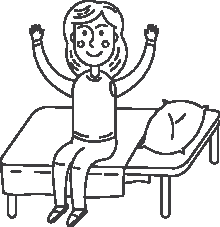
\includegraphics[scale=1.5]{willpower/ch6/1.pdf}
\end{figure}

\subsection*{Кепскі дзень}

Раніцай вам цяжка прачнуцца, вы пераводзіце будзільнік некалькі разоў, устаяце разьбітыя й нясьвежыя. Сьвятло рэжа вочы, і вы не рассоўваеце шторы. Няма апэтыту і жаданьня нешта рабіць. Уся раніца ідзе на тое, каб кафэінам, цукрам і інтэрнэт-серфінгам падняць сабе тонус. Бліжэй да абеду вы ўжо можаце працаваць, але ўзровень энэргіі нестабільны, вам складана доўга канцэнтравацца. Жаданьня выходзіць на вуліцу няма. К вечару хочацца забаваў, вы гледзіце сэрыялы або сядзіце ў~сацсетках. Уначы жаданьня заснуць не зьяўляецца, але розумам вы разумееце, што час ужо ісьці ў~ложак. Кладзяцеся спаць позна, доўга ня можаце заснуць, сьпіце неспакойна.

Немагчыма намаганьнем волі падняць сваю энэргічнасьць ці прымусіць сябе добра спаць. Трэба так арганізаваць свой рэжым і навакольнае асяродзьдзе, каб яны падзаводзілі ваш унутраны гадзіньнік кожны дзень. У гэтым разьдзеле мы гаворым пра тое, як забясьпечыць сабе здаровы сон, сынхранізаваць усе гадзіньнікі свайго арганізма~--- ад сьветлавых і тэмпэратурных да пэрыфэрычных гадзіньнікаў печані, кішачніка, цягліцаў і тлушчавай тканкі.

\subsection*{Дэфіцыт сну}

Ці сталі б вы самі сябе катаваць? Адыліж многія людзі робяць гэта штодня, калі недасыпаюць. Катаваньне бессаньню~--- адно з~самых жорсткіх, прыводзіць да галюцынацыяў і пакутаў. Некаторыя інквізытары аддавалі ёй перавагу, бо яна не пакідала сьлядоў на целе, але людзі былі гатовы прызнацца ў~чым заўгодна. Для нас сон зьяўляецца ня проста адпачынкам, але й найважнейшым, хоць і нябачным, кампанэнтам здароўя. Няма ніводнага органа і фізыялягічнага працэсу, які быў бы незалежны ад сну. 

\infobox{Якасны сон зьяўляецца такім эфэктыўным лекам, што многія праблемы са здароўем могуць быць вырашаныя «праз пасьцелю». З чым бы ні прыйшоў да мяне чалавек, мы абавязкова гаворым і пра сон.}

«Нішто так не ўпрыгожвае чалавека, як васьмігадзінны сон»~--- нібы гэта жарт, але мы сапраўды можам адразу ўбачыць нявыспанага чалавека. Ён дрэнна выглядае, апухлы і крыху пакамечаны, няўважлівы, раздражняльны, безуважлівы. Дасьледаваньні паказваюць, што людзі зь недасыпам здаюцца нам менш прывабнымі, зь імі менш хочацца камунікаваць. \textbf{Дэфіцыт сну зьніжае ўсе нашыя рэзэрвы}: мы павольней рухаемся, пераядаем, становімся адчувальнейшымі да стрэсу, горай цямім і выглядаем старэйшымі. І галоўнае~--- зьніжаецца ўсьвядомленасьць, таму мы папросту не заўважаем у~сабе гэтых зьменаў.

Чалавечы арганізм навучыўся падладжвацца пад цыклі дзень-ноч, каб аптымізаваць свой мэтабалізм і жыцьцядзейнасьць. Днём мы ямо, рухаемся, думаем, а~ўначы адпачываем, перазагружаем і чысьцім мозг, аднаўляемся. Для забесьпячэньня максімальнай эфэктыўнасьці нам патрэбная траціна содняў падрыхтоўкі і адпачынку.

\textbf{Cон~--- гэта таксама праца.} Так-так, сон~--- гэта не пасіўны працэс у~выглядзе ляжаньня на канапе, гэта актыўная дзейнасьць. Сон складаецца з~асобных цыкляў, якія спалучаюць хуткія і павольныя фазы. Падчас павольнага сну адпачывае і аднаўляецца цела, а~ў мозгу адбываецца перанос кароткачасовай памяці ў~доўгачасовую. Падчас хуткага сну актыўны таламус, адбываецца апрацоўка чаканьняў, успаміны перажываюцца нанова, і мы бачым яркія сны, дзе зьмешваюцца рэальнасьць і выдумка, мінулае й будучыня, страхі і задавальненьні. \textbf{Некаторыя аддзелы мозгу працуюць пры гэтым нават больш актыўна, чым пры няспаньні.}

Кіруе сном і цыркаднымі (содневымі) біярытмамі цэлы шэраг мэханізмаў, самым важным зь якіх зьяўляецца супрахіязматычнае ядро гіпаталямуса. У ягоных нэўронах ёсьць пэўныя гены, якія цыклічна кадуюць сінтэз бялкоў CLOCK, BMAL1, PER 1--3. Зьмена канцэнтрацыі гэтых бялкоў уплывае на зарад клеткавай мэмбраны нэўронаў, што вядзе да пэрыядычнай генэрацыі імпульсу. Такая цыклічная актыўнасьць нэўронаў вызначае і ваганьні тэмпэратуры цела, і канцэнтрацыю шматлікіх гармонаў.

\emph{Працягласьць аднаго цыклю сну складае ў~сярэднім 90 хвілінаў. Цыклічная актыўнасьць паўшар'яў мозгу і дынаміка паказьнікаў многіх органаў вагаецца з~цыклем даўжынёй у~90 хвілінаў (да 110--120 хвілінаў у~розных людзей). Ёсьць меркаваньне, што падобныя 90-хвілінныя цыклі актыўнасьці характэрныя і для пэрыяду няспаньня. Кожны такі цыкль складаецца зь 70 хвілінаў актыўнай фазы і 20 хвілінаў пасіўнай, у~тым ліку таму рэкамэндуецца працаваць зь перапынкамі, у~сярэднім раз на гадзіну. І невыпадкова сярэдняя працягласьць аднаго фільма ўсталявалася акурат на адзнацы ў~90 хвілінаў.}

Сон~--- гэта біялягічная патрэба і права. Сёньня мы бачым эпідэмію парушэньняў сну, якія несумненна зьяўляюцца «хваробай цывілізацыі». Недасып адымае энэргію, прадуктыўнасьць, кароціць жыцьцё і павялічвае рызыку мноства захворваньняў. Здаровы сон~--- гэта падмурак здароўя, дабрабыту, прывабнасьці й посьпеху.

\subsection*{Пытаньні і заданьні}

1. Ці лічыце вы свой сон добрым?

2. Як вы пачуваецеся пасьля недасыпу?

3. Ці адчуваеце вы сябе сьвежым пасьля сну?


\section{Сон як новая раскоша: эвалюцыя сну}

Салодкі ціхмяны сон~--- гэта безумоўная прыкмета здароўя. Але ў~сучасным жыцьці ён сустракаецца ўсё радзей: парушэньні сну~--- прыкмета цывілізацыі. У плямёнаў паляўнічых-зьбіральнікаў бессані не сустракаецца, у~іх мовах няма нават словаў для абазначэньня такой зьявы. Толькі 1,5--2,5\,\% зь іх не маглі заснуць уначы часьцей, чым раз на год. 

\infobox{Параўнайце гэта з~хранічнай бессаньню, якая мучыць на працягу жыцьця ад 10 да 45\,\% людзей у~разьвітых краінах.}

Лічыцца, што нашыя продкі спалі даўжэй, дакладней і лепей за нас, засынаючы з~заходам сонца і прачынаючыся на досьвітку. Часткова гэта праўда, часткова выдумка. У сучасных плямёнаў агульная працягласьць сну складае 5,7--7,1 гадзіны, зімой сон даўжэйшы на 53--57 хвілінаў праз падаўжэньне цёмнага часу содняў. Вельмі важная якасьць сну, а~ня толькі ягоная працягласьць.

Цікава, што і раней былі як «совы», так і «жаўрукі», але хранатып часьцей за ўсё мяняўся з~узростам: маладыя «совы» па меры сталеньня становяцца «жаўрукамі». Гэта спрыяе натуральнаму падзелу працы~--- пакуль моладзь сьпіць, дарослыя займаюцца справамі. Навукоўцы называюць гэтай «гіпотэзай бабулі, якая дрэнна сьпіць», так што гэта ня бессань раніцай, а~ваш мозг прачынаецца, каб не дапусьціць нападу драпежнікаў на стойбішча, пакуль моладзь сьпіць.

Ніколі ў~плямёнах не было такога, каб усе спалі~--- амаль заўсёды нехта ня спаў. У любы час ночы адначасова ня спалі як мінімум восем дарослых чалавек. Навукоўцы назвалі гэта «\textbf{гіпотэзай вартавога}», калі гетэрагеннасьць генаў і асынхроннасьць сну дапамагае быць усяму племю напагатове. Гэта ўласьціва ня толькі людзям: напрыклад, сурыкаты таксама заўсёды выстаўляюць «вартавога».

Розныя плямёны кладуцца спаць і ўстаюць раніцай па тэмпэратуры, а~не па сонцы. Так, абуджэньне здараецца ў~пункце мінімальнай тэмпэратуры навакольнага асяродзьдзя. Пры гэтым тэмпэратура кончыкаў пальцаў зьніжаецца, а~вось прыток крыві да мозгу павялічваецца, узровень картызолу таксама расьце.

\emph{Паляўнічыя-зьбіральнікі мала сьпяць удзень (толькі 7\,\% дзённага часу было выдаткавана імі на сон) і ня сьпяць бімадальна~--- гаворка пра начны сон, пабіты пэрыядамі актыўнасьці. Увечары жыхары плямёнаў гутараць, танцуюць, сьпяваюць, любяць спаць разам, вялікімі групамі пад трэск вогнішча і дыханьне супляменьнікаў. Пастаянны рэжым рэгулярна парушаецца: прыкладна раз на месяц ладзіцца «баль», калі адбываюцца шаманскія абрады, танцы, забаўкі. Начныя размовы, як правіла, прысьвечаныя таму, з~чым людзі не датыкаюцца ў~паўсядзённым жыцьці,~--- гэта міты, гісторыі, аповеды пра продкаў.}

\textbf{Зьмяненьне асяродзьдзя.} Праблема са сном і цыркаднымі біярытмамі зьявілася, калі мы змаглі кіраваць асьвятленьнем і тэмпэратурай паветра па-за залежнасьцю ад іх сутачных ваганьняў. Вынаходства лямпачкі дало нам сьвятло ў~любы час содняў, сьвятлодыёдныя лямпы забясьпечылі яшчэ больш яркае і ўзбуджальнае сьвятло. Праца ў~памяшканьнях пазбавіла нас яркага сонечнага сьвятла. Цэнтральнае ацяпленьне зрабіла тэмпэратуру ў~доме пастаяннай, бяз содневых ваганьняў. Лядоўня дае нам ежу калі заўгодна, аўтамабіль і разумовая праца пазбаўляюць нас фізычнай актыўнасьці і фізычнай жа стомы, смартфон і тэлевізар гатовыя напампаваць нас трывожнымі навінамі ў~любы час, ноччу ў~нашых спальнях няма поўнай цемры і занадта шмат шуму. Усё гэта прывяло да таго, што наш унутраны гадзіньнік атрымлівае няслушную, узаемавыключальную інфармацыю з~навакольнага асяродзьдзя і пачынае кіраваць унутранымі працэсамі арганізма няправільна. Вынік~--- множныя дэсынхрозы, то бок парушэньні біялягічнага рытму, самымі вядомымі зь якіх зьяўляюцца парушэньні сну.

\infobox{Важна, каб дзень меў структуру, каб раніца, дзень, вечар і ноч адрозьніваліся паміж сабой. Заснуць намаганьнем волі не атрымаецца~--- трэба зьмяніць асяродзьдзе, каб наш мозг атрымліваў правільныя сыгналы.}

\subsection*{Сон для слабакоў ці сон як раскоша?}

Калі ў~пачатку мінулага стагодзьдзя людзі спалі крыху больш за 8 гадзінаў, то цяпер сярэдняя лічба складае 6,7--7 гадзінаў, то бок працягласьць сну зьнізілася амаль на 1/5 частку. Кожны другі чалавек незадаволены тым, як ён сьпіць. Пры гэтым сон успрымаецца як марнаваньне часу, як прыкмета ляноты, папулярныя прымаўкі «сон для слабакоў», «на тым сьвеце высплюся» і г. д.

\textbf{Раней, калі вы не дасыпалі, гэта як бы служыла прыкметай вашай занятасьці, запатрабаванасьці.} Такі стыль паводзінаў нават атрымаў назву «сонны мачызм». Але сёньня ўсё наадварот: дазволіць сабе не сьпяшацца, спаць столькі, колькі трэба, зьяўляецца прыкметай дастатку і посьпеху. «Салодкі сон у~таго, хто працуе, ці мала ён есьць, а~ці многа; а~сытасьць багатаму спаць не дае»,~--- сказана ў~Бібліі, але сёньня бессань часта мучыць людзей беспрацоўных, бедных, самотных і зь нізкім узроўнем адукацыі. Гэта можа быць зьвязана з~больш высокім узроўнем стрэсу, пражываньнем у~больш шумных месцах і да т.~п.

\begin{figure}[htb!]
  \centering
  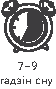
\includegraphics[scale=1.5]{willpower/ch6/2.pdf}
\end{figure}

\subsection*{Недасып}

Колькасьць сну~--- гэта як колькасьць грошай. Ёсьць пражытачны мінімум, а~ёсьць камфортная для жыцьця сума. Так і сон: вылучаюць «ядзерны», працягласьцю 5--6 гадзінаў, які забясьпечвае базавыя патрэбы арганізма, і аптымальны сон працягласьцю 7--9 гадзінаў, які патрэбны для здароўя.

\emph{Занадта доўгі сон таксама зьвязаны з~падвышэньнем рызыкаў. Праблема тут, хутчэй за ўсё, не ў~самой працягласьці, а~ў тым, што за гэтым хаваюцца праблемы са здароўем. Напрыклад, доўгі сон і дзённая дрымотнасьць могуць маскіраваць недых (апноэ), які суправаджаецца нізкай якасьцю сну начнога і частымі абуджэньнямі.}

Праблема \textbf{дэфіцыту сну} яшчэ і ў~тым, што яго немагчыма кампэнсаваць: сонны доўг мае тэндэнцыю назапашвацца незваротна. Калі вы не даспалі тры гадзіны, то на наступную ноч пасьпіце ўсяго на гадзіну даўжэй, то бок дзьве гадзіны сну пайшло ў~дэфіцыт. За бяссонную ноч вы адасьпіцеся ўсяго на тры дадатковыя гадзіны, і чатыры гадзіны сыходзіць у~дэфіцыт. Навукоўцы кажуць пра «сындром недастатковага сну», яго крытэрамі зьяўляюцца: пастаянная дрымотнасьць днём, вы сьпіце менш, чым трэба ў~вашым узросьце, гэта доўжыцца больш за тры месяцы.

Людзі часта спрабуюць падмануць прыроду, спрабуючы кампэнсаваць на выходных свой недасып у~працоўныя дні,~--- гэта нават атрымала азначэньне «сонная булімія» або «сацыяльны джэтлаг», нічога карыснага ў~гэтым няма. Аднак дасьледаваньні паказваюць, што паспаць пра запас усё ж можна: калі вы перад адказнай справай больш пасьпіце, то зможаце паказаць лепшыя вынікі.

\subsection*{Парадокс сну}

Сон~--- як эрэкцыя, чым больш думаеш і турбуесься пра гэта, тым горш становіцца. Калі ў~дасьледаваньнях людзям увесь час нагадвалі, што трэба добра спаць, яны ўсё мацней перажывалі аб якасьці сну, і гэта прыводзіла да больш сур'ёзных парушэньняў сну. Многія людзі ў~звычайным жыцьці пакутліва перажываюць бессань, чакаючы праблемаў з~самаадчуваньнем на наступны дзень.

\textbf{Не намагайцеся заснуць сілаю: прынука толькі ўзмацняе ўзбуджэньне, якое замінае заснуць.} Стаўцеся прасьцей: «Ну, не магу спаць~--- значыць, ня буду». Паляпшаючы сон, важна пазьбягаць напругі й зацыкленьня.

\textbf{Маніторынг сну} і вядзеньне дзёньніка дапамогуць выбраць ідэальныя асабіста для вас вырашэньні праблемы са сном. Існуе вялікая колькасьць фітнэс-бранзалетаў і прыложкавых датчыкаў сну, якія могуць вымяраць структуру сну і нават вызначаць недых. Аднак усе яны маюць розную дакладнасьць і могуць заўважна памыляцца. Захапленьне якасьцю сну можа даходзіць да скрайніх формаў: артасомнія~--- гэта парушэньні сну, выкліканыя празьмерным пра яго клопатам. Памятайце, што нам трэба спаць, каб жыць, а~ня жыць, каб спаць.

\begin{figure}[htb!]
  \centering
  
\includegraphics[scale=1.5]{willpower/ch6/3.pdf}
\end{figure}

\emph{Часам да мяне зьвяртаюцца людзі, зьбянтэжаныя і занепакоеныя зьменамі паказаньняў на датчыках пры адсутнасьці аб'ектыўных крытэраў парушэньняў сну: іх занепакоенасьць часта запускае заганнае кола і сапраўды пачынае замінае ім спаць.}

\subsection*{Пытаньні і заданьні}

1. Зь якімі праблемамі сну вы сутыкаецеся?

2. Што замінае вам спаць? Ці можна гэта ўхіліць?

3. Што дапамагае вам спаць мацней? Ці можна гэта выкарыстоўваць?


\section{Цыркадныя рытмы і дэсынхрозы}

«Засынаю як забіты і прачынаюся як забіты»,~--- скардзіцца мой добры сябар на зьбіты рэжым. Сапраўды, навуковыя дасьледаваньні паказалі наяўнасьць узаемасувязі паміж слушным содневым рытмам арганізма і здароўем чалавека. У выпадку зьбітых біярытмаў~--- калі нашая актыўнасьць высокая і ноччу, і днём,~--- павялічваецца рызыка псыхічных разладаў, уключаючы дэпрэсію і нэўрозы. \textbf{Выбудаваць рэгулярны рэжым сну, харчаваньня, працы і руху будзе вельмі карысна~--- на гэтым грунтуецца ўсё астатняе здароўе.}

\textbf{Сьвятло}~--- гэта ключ, які заводзіць наш унутраны гадзіньнік. У сятчатцы ёсьць адмысловыя клеткі, якія рэагуюць менавіта на зьмену асьветленасьці, на заходы і сьвітанкі. Гэтыя фотаадчувальныя гангліянарныя клеткі працуюць нават у~сьляпых людзей. Дзіўна, але наш цыркадны рытм складае не 24 гадзіны роўна, а~24 гадзіны і 20 хвілінаў. Таму безь сьветлавой падзаводкі нашыя гадзіньнікі могуць занадта моцна сыходзіць наперад.

\textbf{Яркае сонечнае сьвятло} сьцішае выпрацоўку мэлятаніну, гармону сну, а~цемра стымулюе яго выпрацоўку. Таксама важным сыгналам зьяўляецца і тэмпэратура навакольнага асяродзьдзя, бо ўвечары сонца заходзіць і зьніжэньне тэмпэратуры~--- магутны сыгнал для сну. Сваю ролю граюць і пэрыфэрычныя «гадзіньнікі» органаў і сыстэмаў: харчовыя, рухальныя, стрэсавыя.

Таму моцны сон~--- гэта толькі вяршыня айсбэргу, паказьнік нармальнай працы нашых унутраных рытмаў на працягу ўсіх содняў. Пры незбалянсаваным рэжыме дня~--- напрыклад, калі вы працуеце ноччу ці не выходзіце на сьвятло ўдзень,~--- адбываецца дэсынхранізацыя біялягічных рытмаў: разузгадненьне рытмаў арганізма з~рытмамі навакольнага асяродзьдзя з~наступным разузгадненьнем розных рытмаў арганізма паміж сабой. Менавіта таму першае, што трэба рабіць для здароўя,~--- гэта ўсталяваць здаровы рэжым дня, каб сынхранізавана працавалі ўсе вашы ўнутраныя гадзіньнікі: харчовыя, сьветлавыя, тэмпэратурныя, стрэсавыя, цяглічныя.

\begin{figure}[htb!]
  \centering
  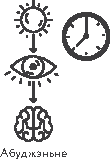
\includegraphics[scale=1.5]{willpower/ch6/4.pdf}\qquad
  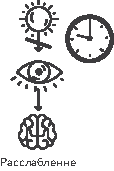
\includegraphics[scale=1.5]{willpower/ch6/5.pdf}
\end{figure}

\emph{Цемра ўключае выпрацоўку гармону мэлятаніну, які стымулюе працэсы аўтафагіі. Але калі вы ясьце ўначы, гэта павялічвае ўзровень гармону інсуліну, што прыгнятае выпрацоўку гармону росту і зьмяншае працэс аўтафагіі.}

\begin{figure*}[htb!]
  \centering
  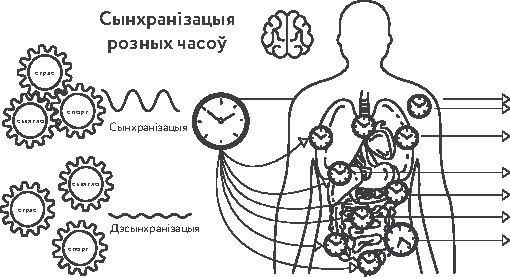
\includegraphics[scale=1.5]{willpower/ch6/6.pdf}
\end{figure*}

\textbf{Дэсынхрозы.} Пры дэсынхрозах узьдзеяньне розных стымулаў адбываецца паапрыч. Пропуск сьняданку, сядзячы лад жыцьця з~самае раніцы, стрэсавая праца~--- усё гэта паступова прыводзіць да разьвіцьця многіх хранічных захворваньняў, ад цукроўкі да дэпрэсіі. Для нармалізацыі біярытмаў раніцай важна на працягу гадзіны пасьля абуджэньня актываваць галоўныя «гадзіньнікі арганізма» з~дапамогай сьвятла, тэмпэратуры, ежы, руху і стрэсу. 

\infobox{Тое, як вы праведзяце першую ранішнюю гадзіну, шмат у~чым паўплывае на ваш настрой днём і на якасьць сну ўвечары і ўначы.}

Мы сутыкаемся зь неабходнасьцю адаптавацца да зьменаў сьветлавога рэжыму кожны год, называючы гэта «восеньскай маркотай» і «вясновым авітамінозам». Зрух рэжыму ўсяго на адну гадзіну хоць і незаўважны для асобнага чалавека, але сур'ёзна ўзьдзейнічае на грамадства ў~цэлым.

\emph{Пераход на летні час, калі мы сьпім на гадзіну менш, прыводзіць да павелічэньня сьмяротных аварый на 6--8\,\% на працягу тыдня пасьля пераводу стрэлак, павышае рызыку інфаркту, суіцыду, частасьць выкліку хуткай дапамогі. А вось пераход на зімовы час, калі мы сьпім на гадзіну больш, зьніжае рызыку інфаркту.}

Дэсынхрозы (рассынхранізацыя) біярытмаў могуць узьнікнуць з~прычыны авіяпералёту і зьмены гадзінных паясоў (джэтлаг), работы па начох, зьменнага графіка. Бывае, што ўдзельнікі працоўнай каманды жывуць у~розных краінах, таму для анляйн-абмеркаваньня праекта трэба адаптавацца да іншага часавага пояса~--- такая сучасная зьява завецца «лічбавы джэтлаг». Распаўсюджаны міт~--- ідэя аб тым, што сон можна чымсьці кампэнсаваць: ежай або дабаўкамі. \textbf{На жаль, гэта не працуе: замены сну не існуе.}

\subsection*{Як старэе наш унутраны гадзіньнік}

З узростам, апроч бачных прыкметаў старэньня, адбываецца і старэньне нашага ўнутранага гадзіньніка. А гэта вядзе да таго, што мяняюцца і пагаршаюцца працэсы, якія ён кантралюе: зрушваюцца пікі ў~амплітудзе ваганьняў тэмпэратуры, мэтабалітаў, гармонаў у~крыві.

\emph{Меншымі становяцца ваганьні тэмпэратуры цела, а~гэта вельмі важна: чым вышэйшая тэмпэратура цела днём, тым больш мы бадзёрыя, чым меншая яна ўначы, тым лепшыя сон і аднаўленьне. Узровень картызолу ўначы становіцца вышэйшым, а~ягоны пік зрушваецца на больш раньні час~--- з~узростам людзі пачынаюць прачынацца ўсё раней, і іх актыўнасьць раніцай вышэйшая.}

Чым выкліканыя гэтыя адрозьненьні? З аднаго боку, гэта працэсы старэньня мозгу і ўжо згаданага супрахіязматычнага ядра; з~другога боку, важным зьяўляецца зьніжэньне адчувальнасьці да сыгналаў, якія кіруюць гадзіньнікам. Напрыклад, наш крышталік, пачынаючы з~18 гадоў, кожны год на 1\,\% страчвае пранікальнасьць, што абмяжоўвае паступленьне сьвятла, асабліва сіняй часткі спэктру, які паляпшае працу гадзіньніка. Як мы ведаем, чым меней сьвятла ўдзень, тым горай працуюць нашыя цыркадныя рытмы. Таму нядзіўна, што выдаленьне катаракты паляпшае мэлятанінавы рытм і, адпаведна, якасьць сну. У адным з~дасьледаваньняў у~дамах састарэлых павелічэньне асьвятленьня днём і зьніжэньне колькасьці сьвятла ноччу ня толькі палепшыла начны сон, але й зьнізіла дзённую дрымотнасьць, палепшыла агульнае самаадчуваньне, павысіла кагнітыўныя здольнасьці.

Па сабе магу сказаць, што сонца~--- вялікі майстар нашых унутраных ключоў. Прытрымлівайцеся здаровага рэжыму дня, правільна сынхранізуйце сьвятло, тэмпэратуру, стрэс, харчаваньне і рух~--- і гэта станоўча паўплывае на працу вашага гадзіньніка і, як вынік, усяго арганізма.

\subsection*{Прынцып рэжыму і сынхранізацыі}

Умацаваньне здароўя патрабуе надзейнага падмурка~--- структураваньня часу. Распарадак дня ляжыць на чатырох краевугольных камянях: гэта рэжым сну, ежы, рухальнай актыўнасьці і працы. Калі вам удалося стварыць свой рэжым дня і датрымлівацца яго, то большую частку працы вы ўжо выканалі. \textbf{Выбудаваны рэжым паступова ўвойдзе ў~звычку і будзе служыць каркасам для здароўя ў~цэлым.}

\emph{Лад жыцьця ў~шматлікіх доўгажыхароў просты і прадказальны: напрыклад, пастухі на Сардзініі штодня прачынаюцца рана і выходзяць даглядаць за жывёламі, без адсыпаньня на выходных або позьняга «завісаньня» з~фільмамі ў~пятніцу.}

Наш арганізм любіць прадказальнасьць: унутраны гадзіньнік лепш працуе, калі мы засынаем і прачынаемся ў~адзін і той жа час, наш страўнік і кішачнік загадзя рыхтуюцца да прыёму ежы, таму так важны рэжым харчаваньня. Трэніроўкі больш эфэктыўныя, калі яны праходзяць па раскладзе, а~не выпадкова час ад часу. У сваёй практыцы я пераканаўся, што без рэжыму нават найлепшыя пачынаньні вырачаныя. Напрыклад, у~зьмене харчаваньня спачатку важна выправіць рэжым, а~ня брацца адразу за зьмену прадуктаў ці зразаньне калярыйнасьці.

Цяпер багата ў~каго бывае пераменны графік працы, частыя вячэрнія забаўкі, пад'яданьні на хаду~--- усё гэта вядзе да таго, што рытм жыцьця становіцца рваным, хаатычным. У адзін дзень чалавек пераядае, у~іншы пералежвае, у~трэці~--- недасыпае і спрабуе гэта кампэнсаваць у~іншы час. Усё гэта~--- кепская ідэя. 

Імкніцеся да таго, каб падтрымліваць рэжым харчаваньня, сну, руху, стрэсу і адпачынку, незалежна ад дня тыдня ці сэзону. Такі лад жыцьця дазволіць вам захаваць здароўе нават у~моманты моцных нагрузак. Пры гэтым манатоннасьць жорсткага рэжыму валодае дэтрэніроўным эфэктам, пазбаўляючы нас карысных стрэсаў. Так, манатоннае харчаваньне прыводзіць да мэтабалічнай адаптацыі да дыеты, калі яна перастае працаваць. У занятках спортам праграма практыкаваньняў непазьбежна страчвае сваю эфэктыўнасьць, бо арганізм да яе прыстасоўваецца. \textbf{Рэдкія парушэньні рэжыму могуць пайсьці на карысьць як разнавід карыснага стрэсу~--- гармэзісу.}

Чым мацнейшая трэніроўка, тым даўжэйшае аднаўленьне, а~новую трэба заплянаваць у~пункце супэркампэнсацыі. Яшчэ старажытныя грэкі, трэніруючы атлетаў, адзначылі магчымасьць павелічэньня прадукцыйнасьці за кошт правільнага чаргаваньня актыўнасьці й адпачынку. Правільнае чаргаваньне розных фізыялягічных станаў важнае для здароўя. Мае сэнс цыкляваць сваю актыўнасьць у~залежнасьці ад гадавога сэзону: улетку, пры высокім узроўні сьвятла, мы можам дазволіць сабе больш вугляводаў, а~ўзімку, калі рухаемся менш,~--- больш тлушчаў, а~вугляводы варта зрэзаць. Пэрыядычны пост (фастынг) хаця і парушае рэжым, але ў~цэлым карысны. Усё гэта будзе ўплываць на якасьць сну.

\subsection*{Пытаньні і заданьні}

1. Ці выконваеце вы штодзённы рэжым харчаваньня (яда прыблізна ў~адзін і той жа час), сну, руху?

2. Ці ўдаецца вам сынхранізаваць харчаваньне, рух і стрэс?

3. Ці адаптуеце вы свой рэжым да іншых зьменаў у~вашым ладзе жыцьця?


\section{Чым небясьпечны дэфіцыт сну?}

Траціну жыцьця мы праводзім у~сьне, і гэтая траціна моцна ўплывае на тое, як мы чуйнуем. Калі вы сёньня трывожныя, нягеглыя і марудлівыя, то, магчыма, рэч проста ў~недасыпе. Пры дэфіцыце сну кагнітыўныя здольнасьці і ўсьвядомленасьць зьмяншаюцца першымі, як і настрой і рухальныя здольнасьці, але мы часта недаацэньваем гэтыя зьмены. Калі сон карацейшы 7 гадзінаў, то гэта можа ў~2,5 разы павялічваць рызыкі розных захворваньняў~--- атлусьценьня, дыябэту, дэпрэсіі, хваробы Альцгаймэра і іншых, і пагаршаць іх цячэньне. 

\emph{Недахоп сну ўплывае на актыўнасьць генаў: актыўнасьць значнай часткі (711 генаў!) была дэфармаваная з~прычыны недасыпу.}

\subsection*{Мозг і кагнітыўныя здольнасьці}

Дэфіцыт сну зьніжае кагнітыўныя здольнасьці: мы на 40\,\% горш запамінаем інфармацыю і асвойваем новыя навыкі. Людзі з~частымі парушэньнямі сну робяць нашмат больш памылак на працы. 

\textbf{Сон павялічвае нэўраплястычнасьць, што дапамагае нам эфэктыўней адаптавацца да нечаканых сытуацыяў.} Кіроўцы, якія ня выспаліся, вельмі няўважлівыя: у~людзей зь бессаньню рызыка трапіць у~аварыю ў~7 разоў большая, чым у~тых, хто нармальна сьпіць. У цэлым больш за 20\,\% аварый адбываюцца праз дрымотнасьці кіроўцаў. Калі ласка, калі вы адчуваеце выразную дрымотнасьць~--- вашыя думкі блукаюць, вам цяжка сканцэнтраваць увагу, вы часта пазяхаеце, -- не сядайце за стырно!

Недасып~--- сур'ёзная перашкода на шляху фармаваньня карысных звычак, затое выдатны каталізатар шкодных: пры недахопе сну чалавек шукае вонкавыя стымулятары, напрыклад кафэін, нікатын, цукар і гэтак далей. Нявыспаны чалавек запальчывы, раздражняльны і пакрыўджаны на ўвесь сьвет. 

\infobox{Недахоп сну зьніжае даступнасьць дафамінавых рэцэптараў у~мозгу, што прыводзіць да імпульсіўнасьці і прыняцьця горшых рашэньняў, меншай задаволенасьці жыцьцём, больш пэсімістычнага сьветаўспрыманьня.}

Чым меней мы сьпім, тым меншая наша стрэсаўстойлівасьць. Так, скарачэньне сну ў~два разы павышае ўзровень картызолу да вечара наступнага дня на 37\,\%. Многія гены, зьвязаныя з~парушэньнямі сну, павялічваюць і рызыку дэпрэсіі: невыпадкова лячэньне дэпрэсіі можа прыкметна палепшыць якасьць сну і наадварот. Парушэньні сну прыводзяць да хваробаў, а~хваробы ўзмацняюць парушэньні сну~--- чарговае заганнае кола. Няпаўнавартасны сон ставіць пад пагрозу ўсе нашыя спробы зьмяніцца і паздаравець, бо ў~гэтым выпадку мы маем горшы самакантроль, пераядаем, прапускаем спартзалю. Дэфіцыт сну ўзмацняе цягу да харчовай узнагароды, прычым нявыспанаму чалавеку перапрацаваная ежа здаецца нашмат смачнейшай, чым таму, хто сьпіць добра.

\subsection*{Імунітэт}

Недасып адмоўна ўплывае на працу імуннай сыстэмы, павялічваючы ўзровень хранічнага запаленьня. Калі сон скараціць напалову, то актыўнасьць проціпухлінных клетак падае на 70\,\%. Для шэрагу разнавіднасьцяў раку дэфіцыт сну зьяўляецца чыньнікам рызыкі: гэта, напрыклад, рак кішачніка, падкарэньніцы і грудзей. Нават эфэктыўнасьць вакцыны меншая, калі рабіць прышчэпку чалавеку, які ня выспаўся.

\subsection*{Цела}

Недахоп сну зьніжае адчувальнасьць да інсуліну, зьніжае гармон сытасьці лептын і павышае гармон голаду грэлін. Чым менш вы сьпіце, тым імаверней зьясьце больш на наступны дзень, а~гэта павялічвае рызыку атлусьценьня і цукроўкі. Калі вы трэніруецеся, то дэфіцыт сну можа зьвесьці на нішто ўсе вашыя намаганьні, затармазіўшы цяглічны рост. Таму так важна пасьля інтэнсіўных нагрузак спаць болей~--- для аптымальнага аднаўленьня.

У мужчынаў, якія сьпяць мала, узровень тэстастэрону адпавядае ўзросту на дзесяць гадоў старэйшаму. У жанчынаў дэфіцыт сну таксама парушае працу палавых гармонаў, зьмяншае лібіда. Пастаянны недахоп сну паскарае старэньне арганізма ў~цэлым і старэньне скуры ў~прыватнасьці. У кантрактах з~мадэлямі агенцтвы пазначаюць у~якасьці абавязковага пункту добры сон, і гэта не выпадкова. 

\emph{Як паказалі дасьледаваньні, ужо пасьля першай бяссоннай ночы ў~скуры зьніжаецца колькасьць вільгаці, зморшчыны глыбеюць, узмацняюцца лушчэньне й чырвань, зьніжаецца элястычнасьць. Да таго ж чым мацнейшы дэфіцыт сну, тым выяўнейшыя праявы на скуры.}

Наагул з~узростам якасьць сну пачынае мець усё важнейшае значэньне, бо структура сну парушаецца, і нам пачынае бракаваць павольнага сну, а~гэта значыць, што горш адбываецца ўзнаўленьне. 

\infobox{Чым старэйшым вы становіцеся, тым больш увагі надайце якасьці сну.}

\subsection*{Якасьць сну} Начныя раздражняльнікі (шум, сьвятло, тэмпэратура) часта парушаюць сон, фрагмэнтуюць яго, выклікаюць мікраабуджэньне, якія мы потым ня можам згадаць. Так, нам здаецца, што мы абвыкаем да шуму ўначы, але ў~рэальнасьці ён кожную ноч дзейнічае на наша цела нэгатыўна, выклікаючы падвышэньне ціску і стымулюючы актыўнасьць стрэсавай сымпатыйнай сыстэмы.

\subsection*{Пытаньні і заданьні}

1. Ці часта вы ў~дрымотным стане кіруеце аўтамабілем?

2. На якую ежу вас цягне пры недахопе сну? Як вы кантралюеце апэтыт?

3. Як вы выглядаеце пасьля недасыпу? Зрабіце фота і параўнайце з~добрай ноччу.


\section{Вечаровае і начное сьвятло}

У «царства Марфэя» вядзе брама з~дзьвюма форткамі: на наступленьне сну ўплывае як працэс стомленасьці~--- або «ціск сну»,~--- так і цыркадныя біярытмы. Кожны з~гэтых працэсаў можа быць парушаны рознымі спосабамі. Ціск сну аслабляецца лішкам кафэіну, высокім узроўнем стрэсу, недахопам рухальнай актыўнасьці. Парушыць цыркадныя біярытмы можна яркім сьвятлом, тэмпэратурай, позьняй вячэрай і да т.~п. Таму й спосабы паўплываць на сон мы разгледзім у~адпаведнасьці з~гэтымі чыньнікамі. Паводле Бібліі, стварэньне сьвету пачалося з~«адзьдзяленьня сьвятла ад цемры». Так і мы пачнём абмеркаваньне чыньнікаў, якія ўплываюць на сон, менавіта са сьвятла~--- галоўнага цыркаднага чыньніка, які кіруе нашым унутраным гадзіньнікам.

\textbf{Сонечнае сьвятло~--- гэта крыніца жыцьця} і сыгнал для нашага ўнутранага гадзіньніка, але лішак сьвятла сур'ёзна шкодзіць нашаму сну. \textbf{Адсутнасьць сьвятла}~--- гэта таксама важны сыгнал для арганізма для падрыхтоўкі да сну, які стымулюе выдзяленьне гармону цемры~--- мэлятаніну.

Вясёлка, якую вы бачыце пасьля дажджу, зьяўляецца, калі белае сьвятло раскладаецца ў~спэктр кроплямі дажджу і паказвае нам сваю прыроду, хвалі рознай даўжыні. Хваля пэўнай даўжыні мае пэўны колер. На адным канцы спэктру~--- чырвоны, ён лёгка ўспрымаецца і слаба дзейнічае на нашы ўнутраныя гадзіны, на іншым канцы~--- высокаэнэргетычнае сьвятло сіняга спэктру, ён аказвае мацнейшае ўзьдзеяньне на наш мозг, прыгнятае выпрацоўку мэлятаніну.

Наш унутраныя гадзіньнік увечары чакае такой жа сьветлавой карціны, як і ў~прыродзе: плыўнага пераходу да вечаровага няяркага нізкага чырвонага сьвятла (як на заходзе сонца) і затым да поўнай начной цемры. Зьніжэньне яркасьці сьвятла таксама памяншае выпрацоўку картызолу, расслабляе, зьніжае апэтыт. Яркае вечарновае сьвятло, асабліва сьвятлодыёднае, з~высокай актыўнасьцю сіняга спэктру, прыгнятае выпрацоўку гармону сну мэлятаніну і парушае працу ўнутранага гадзіньніка. Таму так важна выкарыстоўваць больш здаровыя крыніцы сьвятла, а~таксама абмежаваць выкарыстаньне кампутараў і смартфонаў. Лепей зрабіць гэта як мінімум за дзьве гадзіны да сну, сынхронна зь дзённым часам заходу сонца.

\textbf{Увечары:}
\begin{itemize}
  \item прыглушайце яркае верхняе сьвятло;
  \item выкарыстоўвайце лякальныя крыніцы сьвятла;
  \item пераключайцеся на лямпы напальваньня або іншыя лямпы са спэктрам сьвятла бяз піку ў~сіняй частцы;
  \item не чытайце са смартфона, аддавайце перавагу звычайным кнігам або адмысловым прыладам для чытаньня электронных кніг;
  \item выкарыстоўвайце адмысловыя акуляры (blu-blockers), якія адлюстроўваюць сьвятло сіняга спэктру~--- у~іх вы можаце працягнуць працаваць за экранамі, зьнізіўшы шкоду;
  \item усталюйце праграмы (F.lux і Twilight), якія зьніжаюць яркасьць экранаў і зьмяняюць іх спэктар~--- іх можна наладзіць на аўтаматычнае ўключэньне і выключэньне кожны дзень.
\end{itemize}

\infobox{Для расслабленьня ўвечары можа пасаваць таксама інфрачырвонае сьвятло. Існуюць адмысловыя лямпы і панэлі, зь якімі вы можаце паэкспэрымэнтаваць.}

\emph{Ёсьць шэраг дасьледаваньняў, якія кажуць аб карысьці інфрачырвонага сьвятла для здароўя пры шматлікіх захворваньнях (дыябэт, сардэчна-сасудзістыя і інш.), траўмах (паскарэньне аднаўленьня) і для прыгажосьці (стымуляцыя ўтварэньня калягену ў~скуры, памяншэньне зморшчын), але гэтае пытаньне патрабуе далейшага вывучэньня і больш надзейных доказаў.}

\begin{figure}[htb!]
  \centering
  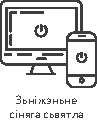
\includegraphics[scale=1.5]{willpower/ch6/7.pdf}
\end{figure}

Калі жывёлы баяцца агню, дык на чалавека агонь аказвае антыстрэсавае ўзьдзеяньне, зьніжаючы ціск і нармалізуючы пульс. Сузіраньне шапаткога, зыркага, жывога вогнішча «паглынае» ўсе пачуцьці~--- слых, зрок, нюх, дотык, прыкоўвае да сябе ўвагу, а, такім чынам, становіцца пэўнага кшталту мэдытацыяй, здольнай зьменшыць неспакой.

\begin{figure}[htb!]
  \centering
  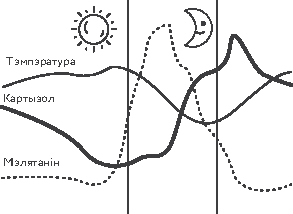
\includegraphics[scale=1.5]{willpower/ch6/8.pdf}
\end{figure}

\emph{Для мяне асабіста гэта адна з~самых расслабляльных працэдураў~--- печка-камін на лецішчы. Калі агмень распалены, цяпло нібыта праймае цябе, выклікаючы расслабленьне й дрымоту, якім немажліва супраціўляцца.}

Homo Sapiens з~самага ўзьнікненьня віду карыстаўся агнём, за сотні тысячаў гадоў да зьяўленьня віду папярэднікі таксама карысталіся агнём. Агонь~--- гэта абарона, ежа, аб'яднаньне, выжываньне для нашых продкаў. Мэханізм дзеяньня полымя складаны: і цяпло, і фрактальнасьць языкоў полымя, і інфрачырвонае выпраменьваньне. Больш за тое, запіс агню на экране таксама працуе.

\subsection*{Начное сьвятло або сьветлавое забруджваньне}

«Паглядзіце на сваю руку ў~спальні. Што вы бачыце?»~--- такім простым спосабам навукоўцы вывучалі сувязь асьветленасьці ў~спальні і рызыкі атлусьценьня. Варыянты адказу: «можна прачытаць тэкст», «можна бачыць супрацьлеглы бок пакоя», «можна бачыць толькі руку», «занадта цёмна, каб бачыць руку». \textbf{Аказалася, што чым сьвятлей у~спальні, тым шырэйшая талія ва ўдзельніц дасьледаваньня.} Пры гэтым ня толькі пакутуе мэтабалізм, але й расьце рызыка паводзінных разладаў і дэпрэсіі.

Навукоўцы называюць гэта сьветлавым забруджваньнем: у~нас шмат лішняга сьвятла як унутры дома, так і ад вулічных ліхтароў. Прыбярыце ці заклейце сьвятлодыёдныя індыкатары тэхнікі, павесьце шторы блэкаўт, калі гэта складана~--- выкарыстайце маску для сну. Маска павінна быць зручнай, ня ціснуць і надзейна трымацца: перабярыце некалькі мадэляў, каб знайсьці аптымальную для вас. Не карыстайцеся начнікамі, а~калі ёсьць неабходнасьць уключыць сьвятло ноччу, то выкарыстоўвайце ў~сьвяцільнях чырвоныя лямпы~--- такое сьвятло слабей за ўсё прыгнятае выпрацоўку мэлятаніну.

Мы недаацэньваем небясьпеку сьвятла нізкай інтэнсіўнасьці. Высьветлена, што начное сьвятло інтэнсіўнасьцью ў~3--5 люкс аказвае нэгатыўнае ўзьдзеяньне на здароўе: для прыкладу, 5 люкс~--- гэта яркасьць невялікай сьвечкі з~адлегласьці 60 см.

\begin{figure}[htb!]
  \centering
  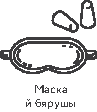
\includegraphics[scale=1.5]{willpower/ch6/9.pdf}
\end{figure}

\subsection*{Пытаньні і заданьні}

1. Купіце акуляры для абароны ад сіняга сьвятла.

2. Выкарыстоўвайце правільнае вечаровае сьвятло.

3. Наколькі цёмна ў~вас у~спальні? Ці бачыце вы сваю руку?


\section{Ранішняе і дзённае сьвятло}

Калі ўвечары і ўначы мы зьніжаем яркасьць сьвятла, то раніцай і днём імкнёмся да яго: для моцага сну і аптымальнага самаадчуваньня нам важна атрымаць дастатковую колькасьць яркага сонечнага сьвятла. Наш унутраны гадзіньнік мае патрэбу ў~вялікай колькасьці сьвятла, бо большую частку часу ў~гісторыі нашага віду мы праводзілі па-за памяшканьнямі.

\emph{У сонечны дзень асьветленасьць дасягае 10\,000 люкс, у~пахмурны дзень~--- 1000 люкс, а~ў нашых дамах і офісах усяго 100--300 люкс.}

Старайцеся бываць на вуліцы ня менш за гадзіну на дзень~--- без сонцаахоўных акуляраў, кепак або капелюшоў. Лавіце сонца праз адчыненыя вокны, праводзіце больш часу на гаўбцы, зрабіце працоўнае месца ля вакна, працуйце тварам да вакна, прыбярыце ўсё, што замінае паступленьню сьвятла: расьліны, жалюзі, шторы. Выкарыстаньне люстэркаў і белага колеру павялічыць асьветленасьць памяшканьня. 

\infobox{У адным з~дасьледаваньняў людзі, якія працавалі каля вакна, атрымлівалі на 170\,\% больш сьвятла, чым тыя, хто сядзеў у~глыбіні памяшканьня, і спалі на 46 хвілінаў даўжэй.}

Калі вы жывяце ў~клімаце, дзе ёсьць праблема зь яркім сонцам, то можна выкарыстоўваць фотатэрапію: набыць і ўключаць з~раніцы на паўгадзіны прыбор зь яркасьцю сьвятла ня менш за 10.000 люкс~--- гэта дапамагае пераадолець восеньскую маркоту і палепшыць сон. У ``цёмны час года'' выкарыстоўвайце сьветлавы будзільнік. Ён здольны плыўна павялічваць яркасьць, імітуючы сьвітанак,~--- і гэта карыснае абуджэньне, бо прачынацца ад званка звычайнага будзільніка ня надта карысна.

Навукоўцы даўно вывучаюць эфэкты сонечнага сьвятла і высьветлілі, што менавіта яркае ранішняе сьвятло~--- самае карыснае для сну і здароўя. Я выходжу раніцай з~дому ў~офіс. Дарога займае каля 25 хвілін ва ўсходнім кірунку, іду амаль насустрач сонцу~--- і гэта вельмі дабратворна ўплывае на маё самаадчуваньне.

\begin{figure}[htb!]
  \centering
  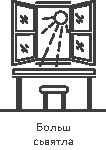
\includegraphics[scale=1.5]{willpower/ch6/10.pdf}
\end{figure}

\emph{Ранішняе сьвятло прыкметна зьніжае сымптомы дэпрэсіі. Дастаткова трох тыдняў ранішняга сьвятла па 30 хвілінаў~--- і частасьць дэпрэсіі зьмяншаецца на 49\,\%! Максімальных значэньняў эфэкт дасягае празь пяць тыдняў. Працуе гэта ва ўсіх узроставых групах.}

Паўгадзіны сьвятла раніцай дастаткова, каб палепшыць вечаровую выпрацоўку мэлятаніну і стымуляваць яго больш раньняе выдзяленьне ўвечары. Таксама сьвятло дапамагае зьменшыць залішні ранішні картызол. Нармалізацыя цыркадных рытмаў станоўча адбіваецца ня толькі на гармонах, але й на абмене рэчываў: ранішняе сьвятло паляпшае адчувальнасьць да інсуліну і дапамагае схуднець. Зьніжэньне вагі пры гэтым невялікае, але яно ідзе выключна за кошт тлушчу, пры гэтым таксама зьмяншаецца апэтыт, асабліва вячэрні. Ранішняе сьвятло прыкметна паляпшае працу мозгу, эфэктыўны пры біпалярных разладх, трывожнасьці. Спартыўныя дасьледнікі таксама выявілі яго станоўчае дзеяньне: паўгадзіны яркага сьвятла раніцай паляпшаюць паказьнікі ў~спартовай стральбе.

\begin{figure}[htb!]
  \centering
  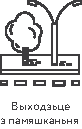
\includegraphics[scale=1.5]{willpower/ch6/11.pdf}
\end{figure}

\subsection*{Пытаньні і заданьні}

1. Як на вас уплывае сьвятло?

2. Ці дастаткова сьвятла раніцай у~вас дома?

3. Калі вы схільныя да восеньскай маркоты, набудзьце лямпы для фотатэрапіі.


\section{Тэмпэратура паветра}

Захутаўся ў~коўдру~--- горача, раскрыўся~--- халодна, высунуў адну нагу~--- ідэальна! Тэмпература цела, навакольнага асяродзьдзя і цеплаабмен паміж імі ўплываюць на наш сон. Ня толькі сьвятло цыклічна зьмяняецца ў~навакольным асяродзьдзі, але й тэмпэратура. Як і многія іншыя біярытмы, тэмпэратура кіруецца содневым цыклем сонца, а~ня ўзроўнем нашай актыўнасьці. Людзі, якія працуюць уначы і сьпяць удзень, дэманструюць той жа цыкл зьмены тэмпэратуры, што і астатнія. Найбольш нізкая тэмпэратура цела адзначаецца раніцай, каля 6 гадзінаў, а~максімальнае значэньне дасягаецца ўвечары, каля 18 гадзінаў. З 19:00 тэмпэратура цела пачынае зьніжацца, дасягаючы найніжэйшага пункту ў~5 гадзінаў раніцы. Зьніжэньне тэмпэратуры цела і навакольнага асяродзьдзя~--- гэта сыгнал да расслабленьня і засынаньня.

Нашыя продкі навучыліся падаўжаць дзень вогнішчам, але й яно паступова згасае, а~начная прахалода вабіць у~ложак. Розныя плямёны ўстаюць і кладуцца спаць па тэмпэратуры, а~не па сонцы: абуджэньне надыходзіць у~пункце мінімальнай тэмпэратуры навакольнага асяродзьдзя раніцай. Пры гэтым тэмпэратура кончыкаў пальцаў зьніжаецца, а~вось прыток да мозгу крыві павялічваецца, узровень картызолу таксама расьце.

\textbf{Што ж адбываецца цяпер?} Цэнтральнае ацяпленьне, цёплае адзеньне, пуховыя коўдры і ваўняныя пледы падтрымліваюць пастаянную тэмпэратуру, гэта перашкаджае астуджэньню цела і замінае заснуць. Даўно забыты такі аксэсуар, як начны каўпак: раней спальні не ацяпляліся, таму каўпак дапамагаў, каб ня мерзьлі вушы. Мы жывём у~пастаянным цеплавым камфорце і развучыліся кіраваць сваім тэмпэратурным рытмам. Пры бессані тэмпэратура цела вышэйшая, і вы напэўна ведаеце, як цяжка заснуць у~сьпякоту. Нават невялікае зьніжэньне тэмпэратуры паляпшае хуткасьць засынаньня і якасьць сну. 

\infobox{Зьніжайце ўвечары тэмпэратуру цела, прыбірайце ўсё, што замінае яму астываць і выводзіць лішнюю цеплыню.}

\emph{Навукоўцы выявілі, што калі нагрэць мозг пацука за ўсё на 0,1\,°С, то ён пачынае пазяхаць, а~пазяханьне вядзе да зьніжэньня тэмпэратуры мозгу. Наш мозг спажывае 25\,\% усёй энэргіі, і яму важна мець надзейную сыстэму астуджэньня для паўнавартаснай работы. Калі мы пазяхаем, то нашая насаглотка запаўняецца халодным паветрам, ніжняя сківіца нацягвае тканкі, адкрываючы доступ у~гаймараву пазуху. Струмень паветра астуджае сьценкі пазухаў і кроў, зьмешчаную там у~крывяносных спляценьнях. А калі сківіцы сьціскаюцца, гэта спрыяе току астуджанай крыві ў~сінусы мазгавой абалонкі. Так, акт пазяханьня астуджае мозг.}

\subsection*{«Трымай галаву ў~холадзе, жывот у~голадзе, а~ногі ў~цяпле»}

У норме мэтабалічная актыўнасьць у~прэфрантальнай кары галаўнога мозгу павінна зьніжацца ўвечары. А вось пры бессані яна застаецца падвышанай. Паніжэньне тэмпэратуры мозгу запавольвае яго мэтабалізм: штучнае невялікае астуджэньне галавы зьяўляецца эфэктыўным спосабам змаганьня зь бессаньню. Нават адна галава над коўдрай дазваляе хутка астываць целу, бо на ёй шмат крывяносных сасудаў, разьмешчаных блізка да паверхні скуры. Цікава, што людзі не дрыжаць, калі холад зьведвае толькі галава.

\begin{figure}[htb!]
  \centering
  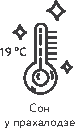
\includegraphics[scale=1.5]{willpower/ch6/12.pdf}
\end{figure}

\textbf{Ахалоньце.} Падчас экспэрымэнту ў~шапачках хворых зь бессаньню цыркулявала астуджаная вада. Вынікі паказалі, што сон паддосьледных амаль нічым не адрозьніваўся ад сну здаровых удзельніц. А для паўнавартаснага сну вельмі важнае чаргаваньне павольнага і хуткага сну, спалучанага з~чаргаваньнем паніжанай і падвышанай тэмпэратуры. 

\textbf{Усё, што замінае нам пазбаўляцца ад цяпла, замінае і заснуць.} Памятаеце гэтае прыемнае адчуваньне, калі гарачая падушка замінае спаць, і вы яе пераварочваеце прахалодным бокам?

Пачніце з~таго, што астудзіце спальню: памяншайце на ноч апал, праветрывайце яе. Аптымальная тэмпэратура ў~спальні складае 18--20\,°С. Прахалоднае паветра астуджае ня толькі галаву, але й цела, бо мы ўдыхаем паветра тэмпэратуры навакольнага асяродзьдзя, а~выдыхаем сагрэтае. Пазбавіцца ад лішняга цяпла можна і з~дапамогай цяпла. Напрыклад, прыміце ванну, яна пашырае сасуды рук і ступняў, тым самым паляпшаючы адвядзеньне цяпла, а~калі вы выходзіце, то эфэктыўна астываеце.

\infobox{Зрабіце лёгкія практыкаваньні да першага поту і ахалоньце, прайдзіцеся ў~лёгкім адзеньні вуліцай, выйдзіце пастаяць на гаўбцы, апранайцеся дома лёгка, кабне замінаць вывядзеньню цяпла.}

Можна выкарыстоўваць грэлку ці шкарпэткі, каб трымаць «ногі ў~цяпле». Сярод сасудаў рук і ног ёсьць вялікая колькасьць тых, што прымае актыўны ўдзел у~тэрмарэгуляцыі. Калі ў~нас халодныя ногі, значыць, сасуды там сьціснутыя, і вывядзеньня цяпла не адбываецца. Халодныя ногі могуць быць прычынай бессані: чым горшы пэрыфэрычны кровазварот, тым часьцей людзі скардзяцца на парушэньні сну.

\emph{Шкарпэткі дазваляюць павялічыць тэмпэратуру ў~пэрыфэрычных частках цела, паляпшаюць якасьць сну, даюць хутчэйшае засынаньне, магчыма, стымулююць выдзяленьне мэлятаніну. Акрамя гэтага, ёсьць і іншыя нечаканыя бонусы: цёплыя шкарпэткі дазваляюць дасягнуць мацнейшага (на 30\,\%) аргазму.}

Выкарыстоўвайце пасьцельную бялізну з~натуральных матэрыялаў, якая добра праводзіць цяпло, выкарыстоўвайце астуджальныя падушкі, цяпер прадаюцца і астуджальныя намартрасьнікі, якія дазваляюць рэгуляваць тэмпэратуру. У дасьледаваньнях устаноўлена, што абцяжараныя да 6--8 кг металічнымі прутамі коўдры на 50\,\% палягчаюць бессань на працягу месяца, а~за год сон нармалізуецца ў~78\,\% пацыентаў, таксама яны палягчаюць сон у~людзей з~трывогай, дэпрэсіяй і біпалярным разладам. Імаверна, што мэханізм дзеяньня абцяжараных коўдраў заключаецца ў~актывізацыі рэцэптараў ціску на скуры, што зьніжае ўзровень стрэсу.

Таксама варта паспрабаваць \textbf{спаць голымі}. Гэта паляпшае вашу тэрмарэгуляцыю, не абмяжоўвае рухі, не замінае лімфаадтоку. Для параў сон галышом паляпшае ўзаемаадносіны, павялічвае ўзровень шчасьця і павялічвае частасьць сэксу.

\subsection*{Начная тэмпэратура}

Аптымальная тэмпэратура ў~спальні на працягу ўсёй ночы дапамагае павысіць якасьць сну, а~акрамя гэтага схуднець і палепшыць мэтабалічнае здароўе нават для цалкам здаровых людзей. У адным з~дасьледаваньняў параўноўваліся дзьве групы здаровых маладых людзей: адны спалі пры 24°C, іншыя~--- пры 19°C. Аказалася, што ўсяго за месяц у~другой групы ў~два разы павялічылася колькасьць бурага тлушчу, які спальвае тлушч з~выдзяленьнем цяпла, і палепшылася адчувальнасьць да інсуліну, што зьяўляецца ахоўнымі чыньнікамі і зьніжае рызыкі захворваньняў.

\subsection*{Ранішняя тэмпэратура}

Зарадка і ўмераная фізычная актыўнасьць раніцай спрыяюць уздыму тэмпэратуры цела і больш высокай актыўнасьці. Дасьледаваньні паказалі, што 20-хвілінная прабежка больш эфэктыўная для павышэньня ўзроўню энэргіі, чым кубак кавы, і парадак у~галаве наводзіць лепш. Я зьяўляюся прыхільнікам бялковага сьняданку, бо бялок валодае найболей высокім тэрмагенным эфэктам у~параўнаньні зь іншымі нутрыентамі. Паўсядзённая фізычная і разумовая актыўнасьці актывізуюцца пры павышэньні тэмпэратуры цела: памятаеце, што пастаянна зьніжаная тэмпэратура цела днём~--- гэта часты сымптом гіпатэрыёзу.

\textbf{Тэмпература ў~доме.} 18\,°С~--- гэта тэмпэратура, пры якой сярэднестатыстычны чалавек можа знаходзіцца працяглы час бязь верхняй вопраткі і шкоды для здароўя. Найбольш спрыяльнай зьяўляецца тэмпэратура, роўная 19--20 градусам. Сардэчна-сасудзістая сыстэма чалавека таксама лепш працуе пры тэмпэратуры ніжэйшай за 22 градусы.

\subsection*{Пытаньні і заданьні}

1. Знайдзіце аптымальны балянс паміж прахалодай і цяплом.

2. Сьпіце ў~прахалоднай спальні.

3. Адрэгулюйце ацяпленьне ў~доме, каб пазьбегнуць завысокай тэмпэратуры.


\section{Рэгулярнасьць засынаньня і абуджэньня}

Засынаньне і абуджэньне~--- гэта працэсы, якім папярэднічае доўгая падрыхтоўка. Напрыклад, узровень гармону актыўнасьці і стрэсу картызолу пачынае паступова падымацца задоўга да таго, як вы прачняцеся. Калі гэты працэс зьбіць, то ёсьць імавернасьць дрэнна засыпаць ці прачынацца «ня з~той нагі». 

\infobox{Рэжым сну стварае адчуваньне ўпарадкаванасьці: навукоўцы высьветлілі, што ёсьць сувязь паміж рытуаламі, зьвязанымі са сном, і задаволенасьцю жыцьцём.}

\textbf{Уставайце заўсёды ў~адзін і той жа час}, незалежна ад таго, працоўны гэта ці выходны дзень. Класьціся спаць таксама важна ў~адзін час, але калі раптам хіліць да сну, то, вядома, варта пайсьці ў~ложак крыху раней. Павольны сон эвалюцыйна больш старажытны, таму пры недасыпе мозг першым кампэнсуе яго дэфіцыт. Калі вы засынаеце, то ў~першай палове сну ён дамінуе, а~колькасьць хуткага сну павялічваецца толькі ў~другой палове сну. Калі вы занадта рана прачнуліся, то пазбавіліся большай часткі хуткага сну.

Карысна сфармаваць \textbf{рэжым здаровага сну}: стварыце вечаровы рытуал, то бок выразную пасьлядоўнасьць дзеяньняў да адыходу да сну. Гэта можа быць што заўгодна (шпацыр, душ, мэдытацыя, дыхальныя практыкі, кніга на ноч і г.~д.), галоўнае~--- штодзённы пастаянны графік. Так вы выпрацуеце звычкі, якія значна палягчаюць засынаньне, і карыстацца такім рытуалам можна будзе ў~новых сытуацыях, калі сон часта бывае клапотны. Часам мы парушаем графік з~добрых прычынаў, напрыклад кладзёмся крыху раней, каб пабольш паспаць. \textbf{Але калі мы не «нагулялі» сон, не адчулі дрымотнасьць, то можам потым доўга валяцца ў~спробе заснуць, а~гэтага рабіць ня варта.}

\begin{figure}[htb!]
  \centering
  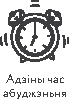
\includegraphics[scale=1.5]{willpower/ch6/13.pdf}
\end{figure}

\textbf{Хранатып.} Які ж ідэальны час засынаньня і абуджэньня? Розны для соваў і жаўранкаў. Аптымальна, калі пэрыяд вашай актыўнасьці супадае са сьветлавым днём. Большасьць людзей могуць лёгка мяняць свой графік, але вось генэтычным «совам» зрабіць гэта цяжэй. Зрэшты, хранатып толькі напалову вызначаецца генэтыкай, а~ўсё астатняе~--- гэта ваш лад жыцьця. Мы можам кіраваць вонкавымі трыгерамі для зьмены цыркадных гадзінаў, каб наладжваць іх найлепшым для сябе чынам. Улічвайце ваш унутраны адказ на рэжым або зрабіце ДНК-тэст~--- на яго аснове можна атрымаць адказ па вашым хранатыпе.

\emph{\textbf{Аналіз ДНК і хранатып.} Падзялюся сваімі вынікамі. У сьніпе (ад анг. Single Nucleotide Polymorphism, SNP, вымаўляецца як «сьніп) rs7221412 у~гене Period 1 у~мяне АА. Значыць, мне зручней уставаць у~сярэднім на гадзіну раней, чым носьбіту варыянту GG.}

\emph{Адным з~галоўных генаў, якія кіруюць нашым унутраным гадзіньнікам, зьяўляецца CLOCK ген. У мяне ў~яго сьніпе rs1801260 вынік СТ (гетэразігота), прамежкавы варыянт. Носьбіты С алелі ў~гэтым сьніпе больш схільныя да дэпрэсіяў, біпалярных разладаў, засынаюць пазьней, маюць больш высокі ўзровень актыўнасьці ўвечары і зьніжаную патрэбу ў~сьне (у параўнаньні з~ТТ).}

\emph{Таксама ў~сьніпе rs228697 у~гене PER3 у~мяне СС, а~кожная алель С павялічвае перавагу ранішняй актыўнасьці. Атрымліваецца, у~мяне відавочна пераважаюць гены «жаўрука», таму і над гэтай кнігай я працую пераважна раніцамі.}

Ёсьць меркаваньне, што аптымальныя для сну гадзіны трапляюць на прамежак паміж 22:00 і 3 гадзінамі ночы~--- у~той час ідзе актыўная выпрацоўка шматлікіх гармонаў. Разумна засыпаць крыху раней, адыходзячы да сну ў~прамежак з~22 да 23:00. Для таго каб гэты час не высьлізгваў ад вас, можна спачатку ставіць будзільнік на 21.30, калі пара прыступаць да «вечаровых рытуалаў» і запісваць час адыходу да сну ў~свой працоўны дзёньнік.

Калі вы ўвесь час прачынаецеся ў~адзін час, то арганізм паступова прыстасуецца пад ваш рэжым. Можна экспэрымэнтаваць, напрыклад, падштурхоўваць час абуджэньня плюс-мінус 15--30 хвілінаў ад звыклага, каб ацаніць, наколькі лёгка вам уставаць. Так можна знайсьці аптымальны для вас час.

\subsection*{Совы мяняюцца}

З досьведу сваёй працы магу ўпэўнена сказаць, што шматлікія людзі, якія лічаць сябе совамі, проста маюць зьбіты графік і лёгка перабудоўваюцца на ранішнюю і дзённую актыўнасьць. Дасьледаваньні паказваюць, што ў~тых месцах, дзе людзі працуюць на вуліцы, роскід паміж совамі і жаўрукамі невялікі, усяго ў~адну-дзьве гадзіны. Мяркуючы са зьвестак генэтыкі, сапраўдных соваў менш за 16\,\%. Сапраўды, дасьледаваньні паказваюць, што, калі совам ссунуць графік, адрэгуляваўшы іх сьветлавы і харчовы рэжымы, то яны атрымліваюць прыкметныя перавагі для здароўя: зьмяншаюцца стрэс і дэпрэсія, паляпшаюцца ня толькі кагнітыўныя, але і фізычныя здольнасьці! Таму для нармалізацыі графіка ўставайце на паўгадзіны раней, кладзіцеся таксама крыху раней~--- і так паступова знойдзеце свой балянс.

\infobox{Даследаваньні паказваюць, што ў тых месцах, дзе людзі працуюць на вуліцы, роскід паміж «совамі» і «жаўрукамі» невялікай, усяго ў адну-дзве гадзіны.}

\subsection*{Рэгулярнасьць часу засынаньня і абуджэньня}

Дасьледаваньні паказваюць, што тыя, хто мала спаў у~будні і адсыпаўся на выходных, выяўлялі горшыя кагнітыўныя здольнасьці, мелі большую вагу і вялікія рызыкі цукроўкі і сардэчна-сасудзістых захворваньняў. Сацыяльны джэтлаг, то бок недасып у~будні і даўжэйшы сон на выходных, зьбівае нашыя біярытмы, павялічвае рызыку дэпрэсіі, частасьць курэньня, ужываньня алькаголю. Калі вы не даспалі, то кладзіцеся раней ці пасьпіце адзін цыкль (паўтары гадзіны) днём. Памятайце, што рэжым~--- перадусім. 

\emph{Калі вы прачынаецеся на выходных нават на адну гадзіну пазьней, гэта павялічвае шанцы атлусьценьня.}

Для падтрыманьня рэжыму важна выкарыстоўваць ложак толькі для сну і сэксу. Ня варта спаць на ложку днём, працаваць і гуляць на ложку, глядзець тэлевізар, размаўляць па тэлефоне, чытаць кнігі, працаваць ці, горай за ўсё,~--- есьці. 

\textbf{Важна класьціся ў~пасьцелю ня проста для адпачынку пры зьяўленьні стомлы, а~толькі калі вы сапраўды хочаце спаць.} Калі вы дрэнна сьпіце, то ня трэба валяцца ў~ложку. Выкарыстоўвайце мэтады кантролю стымуляцыі і абмежаваньня сну.

\textbf{Кантроль стымуляцыі} заключаецца ў~тым, што ня варта ляжаць доўга ў~ложку, калі ў~вас бессань. Гэта важна для тых людзей, хто доўга варочаецца і ня можа заснуць,~--- ложак у~іх пачынае асацыявацца з~пакутлівымі спробамі. Калі ня можаце заснуць 20 хвілінаў, то ідзіце ў~іншы пакой, пазаймайцеся любой спакойнай справай, напрыклад пачытайце. Калі захочацца спаць, зноў вяртайцеся ў~пасьцелю.

\textbf{Мэтад абмежаваньня} сну грунтуецца на ўсталяваньні дакладных часавых рамак. Спачатку неабходна падлічыць рэальную працягласьць сну. Напрыклад, вы спалі 5 гадзінаў, але правялі ў~ложку 8. Значыць, на наступную ноч вам неабходна правесьці ў~ложку ня больш за 5 гадзінаў. Вядома, днём вы будзеце адчуваць дрымотнасьць, але засынаць будзеце хутчэй і спаць мацней. Як толькі якасьць сну палепшылася, падаўжайце пэрыяд знаходжаньня ў~пасьцелі.

\subsection*{Пытаньні і заданьні}

1. Вы жаўрук або сава? Як мяняецца ваш хранатып з~узростам?

2. Прачынайцеся і засынайце ў~адзін і той жа час.

3. Ці ёсьць у~вас рытуалы засынаньня і абуджэньня?


\section{Сьпіце ў~цішыні}

Як толькі ўзьніклі гарады, зьявілася і праблема начнога шуму. На самым пачатку нашай эры рымскі паэт Ювэнал пісаў: «Хворыя тут паміраюць, бо ня могуць спаць. Калі ж прыходзіць сон у~арандаванай хаце? Гэта зусім ня проста, спаць у~гэтым шумным горадзе! Вось чаму кожны тут хворы». Так, ужо ў~Старажытным Рыме былі прынятыя першыя законы, якія забаранялі ўезд вазоў у~начны горад для абароны сну яго насельнікаў. У наш жа час шум атручвае ня толькі сон, але й зьяўляецца самай частай прычынай канфліктаў паміж суседзямі.

Мы нават можам звыкнуць да начнога шуму, але гэта не паменшыць яго шкоднае ўзьдзеяньне на якасьць сну і на арганізм. Для рашэньня праблемы важна выявіць і прыбраць ключавыя крыніцы шуму ўначы: храп партнёра, работа бытавых прыбораў, шум з~вуліцы ці з-за сьцяны.

\emph{Як хуткае рашэньне вы можаце выкарыстоўваць бярушы: лепш за ўсё~--- якасныя васковыя бярушы, якія можна замовіць індывідуальна. Магчыма, варта перабраць некалькі відаў, каб знайсьці анатамічна камфортныя менавіта для вас.}

Зачыняйце вокны~--- тут часта гэта асноўная крыніца шуму. Зачыняйце дзьверы ў~пакой, дзе працуе лядоўня ці кандыцыянэр: шум ад прыбораў не павінны перавышаць 30\,дБ. Можна зьмяніць дызайн кватэры так, каб паменшыць узровень шуму: заплянаваць спальню вокнамі ў~двор, пераставіць мэблю, закрыць шум дываном, ужыць гукаізалюючыя і гукапаглынальныя матэрыялы. 

\infobox{Белы шум ці гукі прыроды могуць палегчыць засынаньне, але сьцеражыцеся белага шуму высокай інтэнсіўнасьці і працягласьці.}

\subsection*{Сон з~партнёрам}

На жаль, партнёр можа быць сур'ёзнай крыніцай шуму і нязручнасьці~--- ад храпу да рухаў цела ў~сьне. Ідэальны выхад~--- спаць у~розных пакоях: гэта забясьпечвае даўжэйшы сон, у~ім у~два разы менш абуджэньняў і на паўгадзіны даўжэйшая фаза доўгага сну. Калі сон сумесны, дык трэба, па магчымасьці, скасаваць усё, што можа перашкодзіць: вялікі ложак і два незалежныя матрацы, шумапаглынальныя дыванкі, бярушы, магчымасьць зручна ўставаць з~пасьцелі для кожнага і да т.~п.

\subsection*{Хатнія жывёлы}

Сабакі і каты рэдка паважаюць ваш рэжым жыцьця, таму практычна кожны другі гаспадар скардзіцца на парушэньні сну. Проста не пускайце гадаванцаў у~спальню. А ў~цэлым хатнія жывёлы, асабліва сабакі, дабратворна ўплываюць на вашае здароўе.

\subsection*{Спальны рыштунак}

Выбірайце для сябе вялікі ложак, дзе вам зручна паварочвацца з~боку на бок. Для матраца важная пругкая падтрымка і магчымасьць зьмяняць позу, не правальваючыся, аптымальнай зьяўляецца сярэдняя жорсткасьць. Выбірайце невысокія падушкі, на якіх зручна захоўваць натуральны выгін шыі,~--- занадта высокія могуць пагоршыць крывацёк. Для пасьцельнае бялізны выкарыстоўвайце натуральныя тканіны~--- яны лепей праводзяць цяпло, менш электрызуюцца і прыцягваюць меней пылу.

\subsection*{Пытаньні і заданьні}

1. Падбярыце сабе зручныя бярушы.

2. Які ўзровень шуму ў~вас у~спальні?

3. Вы храпяце?


\section{Харчаваньне і сон}

«Наемся~--- не магу заснуць, ня ем~--- не магу заснуць ад голаду»,~--- скардзяцца многія. Час, калі мы ямо, уплывае на працу нашых «харчовых гадзінаў», бо адзін з~галоўных гармонаў мэтабалізму інсулін працуе ў~супрацьфазе з~гармонам сну мэлятанінам. Чым больш мы зьядаем на вячэру і чым пазьней вячэраем, тым больш рызыкаў ня толькі для фігуры, але й для сну. Таксама яда на ноч аслабляе працэсы аўтафагіі~--- аднаўленьня і начнога «рамонту» клетак.

Важна \textbf{вячэраць умерана}~--- ня больш за 25\,\% ад сутачнага каляражу, і не пазьней, чым за 3--4 гадзіны да сну. З прадуктаў горш за ўсё на сон уплываюць цукар і рафінаваныя вугляводы. А вось клятчатка ў~гародніне і зеляніне, наадварот, паляпшае якасьць сну і падаўжае фазу павольнага сну. Бялковыя прадукты валодаюць стымулюючым дзеяньнем, таму іх лепей зьядаць на сьняданак, а~не на вячэру. Пазьбягайце прадуктаў, якія зьмяшчаюць аміны (напрыклад, тырамін), які стымулюе выдзяленьне норадрэналіну: гэта сыр, віно, соўсы, паўфабрыкаты, чакаляда.

\begin{figure}[htb!]
  \centering
  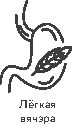
\includegraphics[scale=1.5]{willpower/ch6/14.pdf}
\end{figure}

\emph{Можна прапускаць вячэру, але, калі вы дрэнна кантралюеце апэтыт і голад, то гармон голаду грэлін, які валодае стымулюючым эфэктам, можа пагоршыць засынаньне. У такім разе лепей вячэраць так, каб засынаць без пачуцьця голаду.}

\textbf{Кафэін.} Небясьпечнейшы за ўсё для сну кафэін, ён ёсьць у~каве, гарбаце, многіх ахаладжальных напоях, батоніках. Кафэін і недасып утвараюць заганнае кола: мы горай сьпім, адчуваем дрымотнасьць, п'ём каву, гэта парушае сон на наступны дзень, і так па коле. Кафэін дзейнічае на адэназінавыя рэцэптары ў~мозгу і блякуе сыгналы стомленасьці, маскіруючы зьнясіленьне. Сярэдняе значэньне паўраспаду кафэіну 4--5 гадзінаў, але адмоўна ўзьдзейнічаць на сон ён можа і да 12 гадзінаў.

\begin{figure}[htb!]
  \centering
  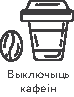
\includegraphics[scale=1.5]{willpower/ch6/15.pdf}\qquad\qquad
  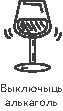
\includegraphics[scale=1.5]{willpower/ch6/16.pdf}
\end{figure}

\emph{Навукоўцы ўсталявалі сувязь паміж ужываньнем кавы, парушэньнямі сну і стомленасьцю па раніцах. А ў~некаторых людзей кава колькасьцю больш за тры кубкі ўзмацняе стрэс, трывогу і нэўроз.}

Правядзіце рэвізію спажываньня кафэіну, складзіце свой «кафэінавы сьпіс». Не ўжывайце кафэінавыя напоі пасьля 14:00 (для некаторых нават пасьля 12:00), прайдзіце кафэінавы дэтокс, адмовіўшыся ад кафэіну на два тыдні, каб ацаніць індывідуальную рэакцыю. Таксама можна зрабіць кафэінавы дэтокс на выходныя.

Памятайце, што кафэін не генэруе энэргію, ён зьнясільвае вас. Кафэін, як і іншыя рэчывы, здольны вырашыць толькі тыя праблемы, якія сам і стварае. 

\infobox{Акрамя кафэіну, шкодны і алькаголь, які моцна зьніжае якасьць сну, узмацняе храп, фрагмэнтуе сон і асабліва моцна парушае фазу хуткага сну. Засынайце цьвярозымі!}

\subsection*{Водны балянс}

Залішняе спажываньне вадкасьці на ноч можа прывесьці да начных абуджэньняў для мочаспусканьня, што пагаршае якасьць сну. У норме павінна быць ня больш за 1--2 мочаспусканьні за ноч. Таму важна за дзьве гадзіны да сну ня піць вадкасьці (за выключэньнем здаволеньня смагі), а~непасрэдна перад сном схадзіць у~прыбіральню. Можна выпіць ня чаю ці кавы, а~зёлкавай гарбаты, многія яе віды расслабляюць і могуць паляпшаць сон (мэліса, мята, чабор, рамонак).

\subsection*{Сындром начнога апэтыту}

Частай прычынай парушэньняў сну зьяўляецца сындром начной ежы. Гэта камбінаванае парушэньне сну і харчаваньня: чым больш калёрыяў вы зьядаеце ўвечары і ўначы, тым горш гэта ўплывае на здароўе. Прыкметамі начнога апэтыту зьяўляюцца скаргі на эпізоды начной ці вечаровай яды, зьніжэньне настрою ўвечары, адсутнасьць апэтыту ранкам. Часта, калі пагаршэньне сну і апэтыту доўжацца ня менш за тры месяцы, гэта спалучаецца зь дзённай стомленасьцю, дэпрэсіяй, пачуцьцём віны. З карэкцыяй такога стану працуе псыхатэрапія, і, вядома, пойдзе на карысьць паляпшэньне рэжыму харчаваньня.

\subsection*{Дадаткі для сну}

Дэфіцыт шматлікіх важных вітамінаў і мінералаў можа пагаршаць сон. Спрыяльна ўплывае папаўненьне дэфіцыту цынку і магнію. Вялікае значэньне маюць вітаміны групы В (B\textsubscript{6}, B\textsubscript{9} і B\textsubscript{12}), прычым папаўняць іх дэфіцыт лепш актыўнымі формамі: пірыдаксаль-5-фасфат, мэтылфалат, мэтылкабаламін. Дадаткі мэлятаніну дапамогуць толькі пажылым людзям або пры зьмене гадзінных паясоў. Паляпшаюць сон шматлікія расьлінныя сродкі: валяр'яна, лаванда, рамонак.

\emph{Зьвярніце ўвагу: шматлікія снатворныя могуць выклікаць залежнасьць, валодаюць мноствам эфэктаў і не захоўваюць нармальную структуру сну. Таму іх можна карыстаць адно ў~выпадку скрайняй неабходнасьці і кароткатэрмінова. Ужываць можна вышэйзгаданыя зёлкі.}

\subsection*{Пытаньні і заданьні}

1. Колькі вы п'яце кавы? Паспрабуйце прыбраць кафэін у~другой палове дня.

2. Падбярыце для сябе расслабляльныя напоі без кафэіну на вечар.

3. Вячэрайце так, каб не адчуваць гострага голаду да засынаньня.


\section{Зьменшыце вячэрні стрэс}

«Меней ведаеш~--- мацней сьпіш»~--- гэтую прымаўку варта згадваць час ад часу. Сапраўды, стрэс зьяўляецца частай прычынай парушэньняў сну. Увечары, калі мы абдумваем праблемы мінулага дня, праз стому ўсё можа здавацца горш, чым ёсьць насамрэч, а~наша рэакцыя на стрэс часта аказваецца небясьпечнейшай за сам стрэсар. 

\infobox{Пракручваньне стрэсавых сытуацыяў у~галаве для нашага цела~--- гэта як шматразовае іх пражываньне нанова.}

Таму важна за пару гадзінаў да сну вылучыць «чысты» час, сказаўшы сабе: «Турбавацца пра гэта я буду заўтра», ну альбо «Пераначуем~--- болей пачуем». Загрузіце свой мозг, займіцеся прыборкай. Паспрабуйце адразу, як скончылі працу, перамыкацца ў~«рэжым адпачынку»: выключайце тэлефон, не заходзьце ў~сацсеткі. Не разважайце пра тое, што не залежыць асабіста ад вас, нават калі гэта значныя рэчы накшталт глабальнага пацяпленьня і курсу валютаў. Адмоўцеся ад прагляду ці чытаньня навінаў увечары, а~мо й ня толькі ўвечары.

\begin{figure}[htb!]
  \centering
  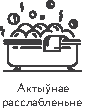
\includegraphics[scale=1.5]{willpower/ch6/17.pdf}\qquad\qquad
  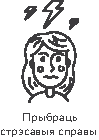
\includegraphics[scale=1.5]{willpower/ch6/18.pdf}
\end{figure}

\textbf{Думайце пра тое, што асабіста вы можаце зрабіць: як смачна павячэраць, з~кім паразмаўляць, што прыгожага надзець і як цудоўна выглядаць.} Адцягвайцеся ад стрэсавых думак музыкай, прыродай, танцамі, цікавай кнігай, падкастам або аповедам. Чытаньне выдатна зьніжае ўзровень гармону стрэсу картызолу, а~чытаньне ўслых мае яшчэ большы расслабленчы эфэкт.

\emph{Шмат хто скардзіцца: «Мне трэба добра выспацца, бо заўтра важны дзень. Але я не магу заснуць, бо заўтра важны дзень». Ня менш за 50\,\% усіх выпадкаў парушэньняў сну зьвязана з~эмоцыямі або стрэсам,~--- так лічаць навукоўцы.}

Антыстрэсавы рэжым, стан спакою вельмі важныя для стварэньня здаровага вечара і мусяць стаць часткай вечаровага рытуалу. Вылучыце гадзіну на клопат пра сябе, пацешце сваё цела і мозг.

\textbf{Усе спосабы расслабленьня можна ўмоўна падзяліць на дзьве групы: зьверху (праз галаву) і зьнізу (празь цела).}

Да \textbf{практыкаў «зьверху»} можна аднесьці чытаньне прыемнай літаратуры, вядзеньне дзёньніка, мэдытацыю, практыку падзякі і спагады~--- яны выдатна расслабляюць. Любыя практыкі ўсьвядомленасьці здымаюць стрэс і паляпшаюць якасьць сну. Яшчэ тысячы гадоў таму ўзьнікла парада «сонца хай ня зойдзе ў~гневе вашым» (Эфэсянаў 4:26).

\emph{Разгрузіце мозг увечары: чым менш у~галаве думак, тым лягчэй засынаецца. Выдатна дапамагаюць розныя тэхнікі накшталт фрырайтынгу, калі вы выпісваеце на аркуш паперы ўсё, што прыходзіць у~галаву. Каб практыкаваньне было карысным, запішыце пляны на заўтрашні дзень~--- паводле дасьледаваньняў, гэта на цэлых 9 хвілінаў паскарае засынаньне.}

Добра зьніжаюць стрэс і \textbf{практыкі «зьнізу»}~--- усе падыходы, якія накіраваныя на цела і актывізуюць блукальны нэрв: масаж, самамасаж, гарачая ванна, расьціраньне, дыхальныя практыкаваньні, саўна і лазьня, касмэтычныя і спа-працэдуры. Доўгі выдых і камфортная затрымка дыханьня на выдыху, глыбокае павольнае дыяфрагмальнае дыханьне~--- дыхальныя практыкі можна рабіць пад кантролем праграмаў.

Ёга, расьцяжкі, пілятэс таксама падыдуць: стрэс узмацняе цяглічную напругу, а~такога роду практыкі дапамагаюць яе зьняць. Можна ўжываць тыбэцкі аплікатар, ролікі па целе, шчотку для цела, абдымкі, аўтагенную трэніроўку, цялесную мэдытацыю, нэрвова-цяглічную прагрэсіўную рэляксацыю~--- усё гэта выдатна працуе.

\infobox{Пазьбягайце спосабаў пасіўнага расслабленьня: ляжаньне перад тэлевізарам, сацсеткі, заяданьне стрэсу і да т.~п. Гэта толькі скрадзе вашу ўвагу й сілы і кепска адаб'ецца на стане здароўя.}

\textbf{Актыўнае расслабленьне} патрэбнае, каб прыбраць застойныя адмоўныя эмацыйныя перажываньні (разумовая жуйка, або румінацыя), калі мы ганяем адны і тыя ж перажываньні па коле. Навукова даведзена, што вядзеньне дзёньніка дапамагае зьменшыць стрэс і палепшыць сон. Таксама можна вылучыць сабе фіксаваны час «пахвалявацца», а~па, скажам, 15 хвілінах больш не вяртацца да гэтых думак. Паспрабуйце пажартаваць зь сябе, абсурдызаваць ці пасьмяяцца з~праблемы. Гіпэрбалізуйце сваё перажываньне~--- пасумуйце хвілінаў пяць ад усёй душы або патрасіцеся ад жаху. Многім людзям не дае заснуць пачуцьцё віны за незавершаныя справы. Раскідайце іх у~штодзёньніку і адпачывайце з~чыстым сумленьнем.

Прыбярыце ўсё, за што чапляецца ваш погляд, навядзіце парадак у~доме і на працоўным стале (пісьмовым і кампутарным). Пачуцьцё завершанасьці дапамагае расслабіцца, невыпадкова пра моцны сон кажуць: «Спіць, як пшаніцу прадаўшы». Вымыйце посуд, выкіньце сьмецьце, падрыхтуйце сумку і адзеньне на заўтрашні дзень, навядзіце парадак вакол і на сваім целе. Усе гэтыя дзеяньні даюць пачуцьцё кантролю і гатоўнасьці, што важна для сну. 

\emph{Спакойная музыка, водары эфірных алеяў, полымя сьвечак~--- усё гэта вы можаце ўключаць у~свой вечаровы рытуал засынаньня.}

\subsection*{Пытаньні і заданьні}

1. Расслабце цела: падыхайце, расьцягніцеся, прыміце ванну.

2. Разгрузіце сабе галаву, запоўніце дзёньнік.

3. Падрыхтуйцеся да заўтрашняга дня.


\section[Актыўнасьць, задавальненьне, дзённы сон і вільготнасьць паветра][Актыўнасьць, задавальненьне і г. д.]{Актыўнасьць, задавальненьне, дзённы сон і вільготнасьць паветра}

Калі мы моцна стамляемся, то патрэба цела ў~адпачынку лёгка занурае нас у~сон. Стаміўшыся фізычна, мы літаральна сьпім хоць зубы выберы: нагрузка паляпшае сон, асабліва яго павольную фазу. Практычна любы від спорту паляпшае сон, але важна, каб вы займаліся даўжэй за 10 хвілінаў, да пачашчэньня пульсу~--- тады і расслабіцца потым будзе прасьцей.

\emph{Ранішняя зарадка~--- найлепшы від актыўнасьці для сну, як ні парадаксальна гучыць. Згодна з~дасьледаваньнямі, тыя ўдзельнікі, хто рабіў практыкаваньні а~7-й раніцы, спалі лепш у~параўнаньні з~тымі, хто займаўся спортам у~13 ці 19 гадзінаў.}

Калі трэніруецеся ўвечары, то не апранайцеся шчыльна і давайце целу астыць пасьля трэніровак~--- гэта дапамагае заснуць. Павольнае кардыё накшталт велатрэнажора, гімнастыкі можна практыкаваць непасрэдна перад сном, а~вось сілавыя, спаборніцкія ці інтэрвальныя практыкаваньні за 2--3 гадзіны да сну лепш пазьбягаць. Расьцяжкі, пілатэс, ёга могуць дапамагчы скінуць цяглічную напругу і спаць мацней.

\begin{figure}[htb!]
  \centering
  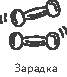
\includegraphics[scale=1.5]{willpower/ch6/19.pdf}
\end{figure}

\textbf{Актыўны спорт на ноч можа толькі пагоршыць сон празь пераўзбуджэньне.} Фізычна актыўныя засынаюць у~сярэднім на паўгадзіны раней, сьпяць на 15 хвілінаў даўжэй і радзей абуджаюцца ў~сьне. Больш за 75\,\% тых, хто пачаў фізычныя практыкаваньні, адзначаюць паляпшэньне якасьці сну. Пры гэтым чым больш у~вашым жыцьці актыўнасьці, тым больш сну трэба для аднаўленьня і цяглічнага росту, а~без дастатковай колькасьці сну фізычныя здольнасьці прыкметна падаюць.

\subsection*{Задавальненьне, пазітыў і сэнс жыцьця}

Пагадзіцеся, што эклер і сэрыял чым пазьнейшыя, тым смачнейшыя. Давайце разьбяромся, чаму так атрымліваецца і як жаданьне «пажыць для сябе яшчэ гадзінку» парушае сон. 

\begin{figure}[htb!]
  \centering
  
\includegraphics[scale=1.5]{willpower/ch6/20.pdf}
\end{figure}

\textbf{Дэфіцыт задавальненьня прыводзіць да дэфіцыту сну.} Калі мы з~розных прычынаў (лішак стымуляцыі, самота, адмова ад хобі і інш.) атрымліваем менш задавальненьня ад жыцьця, наш мозг патрабуе пасьля працоўнага дня атрымаць больш задавальненьня і дафаміну. Зьніжэньне ўзроўню дафаміну парушае рытмы працы ўнутранага гадзіньніка, узмацняе дзённую дрымотнасьць, вядзе да зьяўленьня фрагмэнтацыі сну. Чалавека пачынае нястрымна цягнуць да забаваў увечары, ён імкнецца падоўжыць тое добрае самаадчуваньне, якое ў~яго зьяўляецца, і гэта ўзмацняе недасып. Так узьнікае «адкладзены» стыль жыцьця. Таму так важна спаталяць свой эмацыйны голад прадуктыўна на працягу дня і загадзя прадумваць для сябе задавальненьні, няхай гэта будзе новы фільм і новае месца, хобі і камунікацыя, цікавая кніга і шпацыр.

\infobox{Запішыце тры задавальненьні, якія вы атрымалі сёньня, і абавязкова заплянуйце задавальненьне на заўтра~--- такое чаканьне будзе дабратворна ўплываць на ваша самаадчуваньне.}

\textbf{Больш задавальненьняў.} Каб мацней спаць уначы, трэба болей цешыцца днём. У тых людзей, хто схільны да дэпрэсіі і парушэньняў сну, менш пазітыўных думак і больш нэгатыўных. Карысна прыцэльна працаваць над эмоцыямі і вучыцца шукаць добрае ў~паўсядзённым жыцьці, пераадольваючы прыроджаную схільнасьць фіксавацца на нэгатыве.

\emph{Падумайце, што пазітыўнага і добрага было сёньня? А што пазітыўнага можа адбыцца заўтра? Якія дасягненьні ў~вас сёньня? А чаго вы можаце дасягнуць заўтра? Усё роўна, вялікія ці малыя гэта будуць моманты й посьпехі, важнае адчуваньне вэктару вашага руху. Навукоўцы высьветлілі, што тыя людзі, якія маюць больш ясны напрамак руху ў~жыцьці і ў~якіх ясьнейшыя сэнсы жыцьця, лепей сьпяць.}

\subsection*{Удзячнасьць}

Пачуцьцё ўдзячнасьці й спагады актывуе антыстрэсавую сыстэму і выдатна расслабляе. Пагаварыце з~блізкімі людзьмі, правядзіце зь імі «чысты» час без адцягненьня ўвагі на смартфон. Абдымкі, погляд воч-у-воч, камплімэнты, гумар расслабляюць. Падумайце пра важнае ў~вашым жыцьці, пагартайце дзёньнік. Запішыце сытуацыі, у~якіх вы былі ўдзячныя нечаму ці некаму. Адчуваньне сэнсу пражытага дня важнае, для таго каб пасьпяхова супрацьстаяць бягучым стрэсам.

\subsection*{Сэкс}

Блізкасьць, абдымкі і сэкс важныя для дабрабыту і сну, а~для многіх сем'яў сумесны сон~--- гэта яшчэ адна магчымасьць быць разам. Нават калі вы сьпіце асобна, рэгулярна прыходзьце да партнёра або запрашайце яго ў~сваю спальню. Сэкс прыкметна (на 20\,\%) паляпшае якасьць сну, эндарфіны і аксытацын дапамагаюць у~гэтым. Ранішні сэкс можа быць выдатным пачаткам дня.

\subsection*{Якасьць паветра ў~спальні}

Вы схадзілі ў~прыбіральню, прынялі душ, пачысьцілі зубы~--- спаць у~«цялеснай чысьціні» прыемна. Аднак гэта яшчэ ня ўсе нашы выдзяленьні: мы выдыхаем у~паветра прадукты абмену, часам іх нават называюць «газападобным калам». І днём, і падчас сну мы выдзяляем з~дыханьнем вуглякіслы газ, адзін чалавек за гадзіну выдыхае 30 літраў CO\textsubscript{2}! Куды ж ён зьнікае?

За час сну ў~пакоі 20\,м\textsuperscript{2} прырост CO\textsubscript{2} будзе складаць 500 ppm кожную гадзіну, і калі ў~спальні слабая вэнтыляцыя, то да абуджэньня яго ўзровень у~дзесяць разоў перавысіць норму. Сон у~спальні без вэнтыляцыі з~высокай канцэнтрацыяй вуглякіслага газу прыводзіць да пагаршэньня кровазвароту галаўнога мозгу, стомленасьці, разьбітасьці і раздражняльнасьці, можа ўзмацніць храп, цяжар у~галаве і галаўны боль.

\emph{Важна правяраць з~дапамогай CO\textsubscript{2}-датчыка якасьць паветра і, пры неабходнасьці, выправіць вэнтыляцыю: усталяваць прытокавы клапан паветра, праверыць цягу ў~вэнтшахтах, адчыняць акно на мікраправетрываньне, трымаць дзьверы ў~спальню адчыненымі.}

\begin{figure}[htb!]
  \centering
  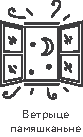
\includegraphics[scale=1.5]{willpower/ch6/21.pdf}
\end{figure}

Асабліва часта вільготнасьць падае зімой праз цэнтральнае ацяпленьне. \textbf{Нізкая вільготнасьць паветра вядзе да перасыханьня дыхальных шляхоў, што вядзе да закладзенасьці носа і павялічвае рызыку ГРЗ.} Таксама сухасьць памяшканьняў павялічвае колькасьць пылу ў~паветры. Выкарыстоўвайце ўвільгатняльнік паветра і падтрымлівайце вільготнасьць у~спальні ня менш за 50\,\%.

\textbf{Чым лепшае паветра (вэнтыляцыя і вуглякіслы газ, дастатковая вільготнасьць, чысьціня), тым меншая рызыка недыху~--- апноэ.} Старыя матрацы і тканіны могуць утрымліваць прадукты жыцьцядзейнасьці пылавых кляшчоў, якія раздражняюць дыхальныя шляхі. Пыл, які асядае на тканінах і абіўках, таксама нэгатыўна ўплывае на дыханьне, таму пэрыядычная ўборка ці выдаленьне падобных пылазборнікаў са спальні станоўча адаб'ецца на якасьці сну.

\emph{Навукоўцы высьветлілі, што чысьціня паветра (колькасьць дробных часьціц P2.5 у~ім) амаль напалову скарачае якасьць сну і выклікае праблемы з~засынаньнем. Паветраны фільтр (HEPA-фільтар) у~вашай спальні будзе здаровым рашэньнем, асабліва калі вы жывяце ў~буйным горадзе ці паветра ў~вашым раёне бруднае (падрабязна пра гэта ў~разьдзеле «Шкоднае асяродзьдзе»).}

\subsection*{Дзённы сон}

Гэта гісторыя пра тое, як нашыя дзіцячыя правілы~--- накшталт шмат гуляць на вуліцы і спаць днём~--- становяцца дарослымі задавальненьнямі. Дзённы сон добры ня толькі ў~дзіцячым садку. У нашым біярытме ёсьць натуральны момант падзеньня актыўнасьці ў~прамежку з~13 да 15 гадзінаў. Прыблізна праз 8 гадзінаў пасьля абуджэньня наш узровень картызолу зьніжаецца, і мы адчуваем стому й дрымотнасьць. Таму ў~некаторых выпадках карысна крыху падрамаць, але ня ўсім і не заўсёды.

\emph{Дзённы сон натуральны для чалавека, яго традыцыя (сіеста, інэмуры) ёсьць у~розных культурах. Дзённы сон павялічвае прадуктыўнасьць на 34\,\% і ўвагу на 54\,\%, паляпшае запамінаньне і кагнітыўныя здольнасьці. 20 хвілінаў сну эфэктыўнейшыя за некалькі кубкаў кавы і дапамагаюць згладзіць наступствы дрэннага сну ноччу. Сіеста нават тры разы на тыдзень на 37\,\% памяншае сьмяротнасьць ад інфаркту і зьніжае рызыку дэпрэсіі.}

Аптымальна паспаць ня больш за 30 хвілінаў, каб не прачнуцца ў~фазе глыбокага сну і ня трапіць пад інэрцыю сну~--- пагаршэньне самаадчуваньня пры абуджэньні ў~глыбокай фазе. Занадта доўгі дзённы сон можа запаволіць засынаньне ўвечары.

Дзённы сон можна практыкаваць у~любым месцы (офіс, дом, машына): стаўце будзільнік, выкарыстоўвайце маску для сну і бярушы. Можна выпіць кубак кавы да дрымоты, і кафэін пачне дзейнічаць акурат пасьля абуджэньня. Пры гэтым дзённая дрымотнасьць на тле нармальнай працягласьці начнога сну можа быць небясьпечным сымптомам недыху, цукроўкі, дэпрэсіі, парушэньня работы шчытавіцы, дэфіцыту жалеза. Выключыце гэтыя станы, не ігнаруйце такога роду дрымотнасьць, не заглушайце яе кафэінам.

\begin{figure}[htb!]
  \centering
  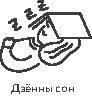
\includegraphics[scale=1.5]{willpower/ch6/22.pdf}
\end{figure}

\textbf{8-гадзінны сон ноччу і 20--30 хвілінаў сну днём у~прамежак ад 13:00 да 15:00~--- гэта, мабыць, самы аптымальны рэжым.}

\subsection*{Пытаньні і заданьні}

1. Заплянуйце сабе задавальненьні на ноч, структуруйце свой вечар.

2. Ці дапамагае вам дзённы сон?

3. Вызначыце ўзровень вільготнасьці ў~спальні. Як можна яго аптымізаваць?


\section{Бессань, недых і дэпрывацыя сну}

Як і са стрэсам, часта неспакой пры парушэньнях сну можа прынесьці больш шкоды для здароўя, чым сама па сабе адсутнасьць сну. Адны людзі прымушаюць сябе заснуць сілай волі і трывожацца з~нагоды наступнага дня, даводзячы сябе да зьнямогі. Іншыя пачынаюць ужываць снатворныя, але ж снатворныя ня лечаць прычыну, якая выклікала бессань, яны пагаршаюць архітэктуру сну, могуць выклікаць залежнасьць і мець заўважтныя пабочныя эфэкты. Той жа мэлятанін не зьяўляецца панацэяй і, на маю думку, можа нават прынесьці шкоду людзям маладога і сярэдняга ўзросту. Нават, здавалася б, бясьпечныя зёлкі, такія як валяр'яна, часам могуць выклікаць парадаксальную рэакцыю.

Няправільна рэагуючы на парушэньні сну, чалавек можа спрыяць разьвіцьцю «навучанай бессані», калі яна становіцца хранічнай. Вы баіцеся недасыпу, баіцеся не заснуць, гэта вядзе да ўзмацненьня ўзрушанасьці, і вы рэальна пачынаеце горай спаць. Важна ставіцца прасьцей, не катастрафізаваць сытуацыі, у~якіх вы ня сьпіце,~--- у~рэшце рэшт, гэта дапаможа лягчэй перажыць бяссонную ноч.

\infobox{Памятайце, што нават у~бяссонныя ночы мы ўсё роўна сьпім больш, чым нам здаецца, бо маем тэндэнцыю прымяншаць колькасьць сну.}

Акрамя першаснай бессані, ёсьць і другасная, выкліканая ўсталяванымі звонку прычынамі. Як толькі яны вырашаюцца, якасьць сну аўтаматычна паляпшаецца. Гэта могуць быць стрэсавыя сытуацыі, стымулятары, захворваньні. Напрыклад, на новым месцы нам бывае цяжка заснуць, але гэта натуральная біялягічная рэакцыя, калі нязвыкласьць і магчымыя небясьпекі прымушаюць наш мозг ня спаць. Многія хваробы выклікаюць праблемы са сном, на першым месцы сярод іх упэўнена стаяць недых і дэпрэсія. Меншы ўплыў на сон аказваюць сындром неспакойных ног, астма, энцэфаліт, хвароба Паркінсана і Альцгаймэра, захворваньні шчытавіцы. 

\emph{Некаторыя сымптомы, напрыклад начная патлівасьць, таксама могуць быць праявай недыху, сухотаў, мэнапаўзы, гіпаглікеміі пры дыябэце, тырэятаксікозе, гастраэзафагеяльнай рэфлюкснай хваробы і да т.~п.}

\textbf{Парушэньні сну бываюць двух відаў}: калі вам цяжка заснуць (парушэньне засынаньня) і калі вы прачынаецеся ўначы і ня можаце заснуць (парушэньне падтрыманьня сну). Цяжкасьці з~засынаньнем часта бываюць зьвязаныя са стрэсавымі прычынамі, а~вось цяжкасьці з~абуджэньнем сярэдначы могуць быць зьвязаныя з~дэпрэсіяй, і часам гэта адзіная праява схаванай дэпрэсіі. У маёй практыцы бывала, што менавіта лячэньне дэпрэсіі прыводзіла да паляпшэньня сну, усе шматлікія спробы палепшыць гігіену сну не ўплывалі на яго якасьць і працягласьць.

\begin{figure}[htb!]
  \centering
  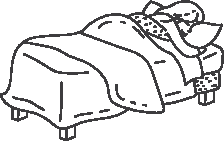
\includegraphics[scale=1.5]{willpower/ch6/23.pdf}
\end{figure}

\subsection*{Недых (апноэ)}

Недых~--- гэта частыя прыпынкі дыханьня ў~сьне і самая частая прычына парушэньняў сну. Недых зьяўляецца цяжкім, але папраўным станам, на жаль, яго часта ня могуць дыягнаставаць. Недых падступны, ён маскіруецца храпам, у~яго мала самастойных праяў, але пры гэтым ён правакуе разьвіцьцё шматлікіх іншых захворваньняў: атлусьценьне, сардэчна-сасудзістыя захворваньні, пашкоджаньні мозгу і інш. Часта да гэтай праблемы дадаюцца начная і ранішняя гіпэртэнзія і вісцэральная атлусьценьне. Начны недых можа зьвесьці на нішто спробы чалавека схуднець, а~вось пасьля яго карэкцыі адбываецца памяншэньне вагі. Павелічэньне абхопу шыі~--- чыньнік рызыкі апноэ. Паводле розных ацэнак, недых можа ўкараціць жыцьцё на 15--20 гадоў, пры гэтым чалавек будзе ўвесь час пакутаваць ад дрымотнасьці, стомы, недахопу энэргіі.

Пры падазрэньні на недых неабходна зьвярнуцца да спэцыяліста для ўдакладненьня дыягназу і лячэньня. Для зьніжэньня храпу не ўжывайце алькаголь, сьпіце на баку, трымайце гігіену дыхальных шляхоў, схуднейце. Ёсьць шмат розных дапаможных прыладаў: налепкі і пластыры на нос, насавыя і ротавыя ўкладышы, якія перашкаджаюць спадзеньню дыхальных шляхоў. Дыханьне праз рот можа пагоршыць сон і нават павысіць рызыку карыесу, адзінкавыя дасьледаваньні гавораць аб магчымай карысьці нават заклейваньня рота на ноч, хоць патрабуюцца дадатковыя дасьледаваньні для праверкі гэтай ідэі. Паменшыць выяўленасьць храпу дапаможа лячэньне захворваньняў і дэфармацый насавой поласьці, трэніроўка цягліцаў глоткі, ніжняй сківіцы і языка, артыкуляцыя, сьпевы, ігра на спэцыфічных інструмэнтах, такіх як дыджэрыду.

Дыягназ ставіцца пры полісамнаграфіі, але неаднаразовыя прыпынкі дыханьня ў~сьне, гучны храп, частыя начныя мочаспусканьні і дзённая дрымотнасьць~--- гэта тыповыя яго прыкметы. Калі ёсьць хаця б адна з~гэтых прыкметаў, неабходна выключыць недых. Некаторыя гаджэты, напрыклад сыстэма для аналізу сну Sleep Analyze (Withings), могуць вызначаць недых.

\subsection*{Нактурыя}

Начныя паходы ў~прыбіральню часьцей за адзін раз (нактурыя)~--- гэта прыкмета парушэньня здароўя. Яны сустракаюцца ў~кожнага трэцяга чалавека старэйшага за 30 і ня толькі зьніжаюць якасьць сну, але й могуць быць прадвесьнікамі многіх захворваньняў. Для больш дакладнага вызначэньня прычынаў варта пэўны час весьці дзёньнік мочаспусканьня~--- адзначаць час і аб'ём кожнага мочаспусканьня, з~указаньнем сілы пазыву, дыскамфорту, неабходнасьці натужваньня і інш. 

\infobox{Сярод адносна дабраякасных прычынаў частых пазываў у~прыбіральню вылучаюць залішнюю водную нагрузку ўвечары, позьняе ўжываньне кафэіну і алькаголю.}

Пачашчэньне начных паходаў у~прыбіральню~--- гэта прыкмета старэньня. Пасьля 50 гадоў падвойваецца колькасьць начной мачы: чым старэйшы чалавек, тым больш мачы выдзяляецца ноччу. Аднак перад тым, як сьпісаць гэта на старэньне, трэба выключыць хваробы: сардэчная і нырачная недастатковасьць, сындром апноэ ў~сьне, цукроўка, гіпэрплязія падкарэньніцы, інфэкцыі мачавых шляхоў, праляпс мачавога пухіра, дэфіцыт андрагенаў.

\subsection*{Бруксізм}

Бруксізм (зубоўны скрогат) можа замінаць сну, але лечыцца ён дастаткова складана. Выкарыстоўваецца набор розных падыходаў~--- ад дадаткаў і зьніжэньня стрэсу да кіраваньня тонусам жавальнай мускулатуры,~--- таму для абароны зубоў ад пашкоджаньня варта выкарыстоўваць спэцыяльныя капы. 

\subsection*{Сындром неспакойных ног}

Сындром неспакойных ног досыць часта мае генэтычную схільнасьць і зьвязаны з~абменам дафаміну. Ліквідацыя правакацыйных чыньнікаў, ад папаўненьня дэфіцыту жалеза да зьніжэньня колькасьці кавы, можа дапамагчы аблегчыць гэты стан. Таксама дапамагае лячэньне спадарожных захворваньняў, адмена лекаў, якія правакуюць гэты стан, і да т.~п.

\subsection*{Дэпрывацыя сну}

Працяглая адсутнасьць сну выклікае захворваньні, але ў~малых дозах дэпрывацыя сну можа быць карыснай. Чалавечая культура з~самых раньніх часоў утрымлівае рытуалы, пэрыядычна выконвальныя ўсю ноч: можна ўспомніць ўсяночныя чуваньні, вігіліі, будыйскі данчод-хурал ды іншыя абрады, якія трываюць да самай раніцы. Яшчэ старажытныя рымляне ведалі, што бяссонная ноч здольная на некаторы час пазбавіць чалавека ад дэпрэсіі. Сапраўды, дэпрывацыя сну дапамагае пры цяжкіх формах дэпрэсіі, якія не адказваюць на антыдэпрэсанты. Незвычайныя адчуваньні пасьля бяссоннай ночы часткова абумоўленыя ўздымам дафаміну.

\textbf{Існуе некалькі хронабіялягічных мэтадаў лячэньня дэпрэсіі}: поўная дэпрывацыя сну, тэрапія абуджэньнем, зрух фазаў сну, калі мы раней кладзёмся, лячэньне сьвятлом і цемрай, лячэньне яркім сьвятлом. Часта выкарыстоўваецца трайная хронатэрапія: спалучэньне дэпрывацыі сну, яркага сьвятла раніцай і раньняга адыходу да сну. 

\emph{Зь немэдыкамэнтозных спосабаў хронатэрапія працуе нават лепш за фізычную актыўнасьць: паляпшэньне ў~41\,\% у~групе дэпрывацыі супраць 13\,\% у~групе трэніровак у~першы тыдзень, 62\,\% супраць 38\,\% праз 28 тыдняў.}

Адсутнасьць сну пасьля гострага стрэсу зьніжае рызыку посттраўматычнага стрэсавага разладу: падчас сну інфармацыя з~кароткачасовай памяці пераходзіць у~доўгачасовую, а~адсутнасьць сну парушае гэты працэс. Бяссонная ноч сьцірае ўспаміны і аслабляе эмацыйную рэакцыю на мінулае. Парадаксальна, але адсутнасьць сну можа дапамагчы вылечыць бессань. Абмежаваньне сну ўзмацняе «ціск сну», таму дрымотнасьць на наступную ноч можа ўзмацніцца. Як асобны мэтад гэта не практыкуецца, але выкарыстоўваецца ў~складзе кагнітыўна-паводзіннай тэрапіі бессані.

\emph{Кагнітыўна-паводзінная тэрапія зьяўляецца адным з~самых эфэктыўных немэдыкамэнтозных спосабаў палепшыць якасьць сну без пабочных эфэктаў. Яе можна праходзіць у~спэцыяліста або карыстацца многімі прынцыпамі самастойна.}

\subsection*{Пытаньні і заданьні}

1. Ці ёсьць у~вас дзённая дрымотнасьць?

2. Ці моцна вы храпяце?

3. Ці часта вы ходзіце ў~прыбіральню ноччу?


\section{Правільнае абуджэньне і раніца}

Засынаньне з~абуджэньнем~--- гэта найважнейшыя складнікі мастацтва моцнага сну. Калі вы ўстаяце «ня з~той нагі», то ўвесь дзень ідзе наўскасяк. А посьпех прыходзіць ня проста да тых, хто рана ўстае, а~хто прачынаецца энэргічным і пазітыўным. \textbf{Сапраўды, як сустрэнеш дзень, так яго і правядзеш.}

Найважнейшымі часткамі дня, якія забясьпечваюць зладжаную працу нашага ўнутранага гадзіньніка, зьяўляюцца раніца і вечар. Адначасовая падзаводка біярытмаў раніцай забясьпечвае нас зарадам бадзёрасьці на цэлы дзень. І наадварот: калі мы выкарыстоўваем розныя стымулы несынхранізавана, гэта можа прыводзіць да парушэньняў працы ўнутраных органаў: пропуск сьняданку павялічвае адчувальнасьць да стрэсу, што можа паўплываць на засынаньне, а~недахоп сьвятла раніцай вядзе да дрымотнасьці.

\subsection*{Ранішняя сынхранізацыя}

Калі людзі кладуцца позна, то раніца для іх пачынаецца стрэсава і ў~мітусьні. Пры гэтым ранішні час самы рэсурсны, таму так важна хаця б паўгадзіны, а~ў ідэале гадзіну, прысьвяціць асабіста сабе: няхай гэта будзе вядзеньне дзёньніка, плянаваньне, мэдытацыя, разважаньні, прыняцьце рашэньняў. Гэта дапаможа вам быць больш усьвядомленымі і сабранымі на працягу дня. Ваша ранішняя гадзіна асабіста для сябе можа быць крытычна важнай для вашага росту. Спытайце сябе раніцай, што добрага вы зробіце сёньня? Што вы зробіце, каб наблізіцца да сваіх мэтаў? А як бы вы правялі гэты дзень, ведаючы, што ён апошні?

\begin{figure}[htb!]
  \centering
  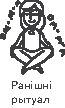
\includegraphics[scale=1.5]{willpower/ch6/24.pdf}
\end{figure}

\textbf{На працягу першай гадзіны пасьля абуджэньня заводзім усе гадзіньнікі нашага арганізма: уключаем яркае сьвятло, прымаем халодны ці кантрасны душ з~расьціраньнем, робім кароткую інтэнсіўную зарадку, шчыльна сьнедаем з~акцэнтам на бялковыя прадукты, вызначаем тры галоўныя задачы на сёньняшні дзень, у~ідэале~--- трохі прайсьціся па дарозе на працу, пабываўшы на сонца. Гэтыя дзеяньні дазваляюць скінуць інэрцыю сну, больш актыўна пачаць свой дзень.}

\subsection*{Вечаровая сынхранізацыя}

Вечаровая сынхранізацыя мяркуе адваротныя ранішняй дзеяньні: зьніжэньне яркасьці сьвятла, памяншэньне стрэсу, манатонныя і расслабляльныя дзеяньні, прахалода і спакой. Для адных такімі манатоннымі дзеяньнямі зьяўляюцца вязаньне ці чытаньне ўслых дзецям. Вельмі часта многія шкодныя звычкі, напрыклад пераяданьне, больш актыўныя ўвечары, калі чалавек стаміўся і ягоная воля аслабленая. Таму так важна мець добры плян дзеяньняў на вечар і вылучыць хоць паўгадзіны «чыстага» часу пабыць сам-насам з~сабою, якасна адпачыць. Без выразнага вечаровага пляну мозг будзе вас спакушаць ня самымі здаровымі варыянтамі.

\begin{figure}[htb!]
  \centering
  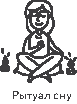
\includegraphics[scale=1.5]{willpower/ch6/25.pdf}
\end{figure}

\emph{Калі раніца больш рацыянальная, то вечар часта бывае больш крэатыўным. Так, аналіз шахматнай гульні паказаў, што, незалежна ад вашага хранатыпу, раніцай стратэгія гульні заўсёды больш абдуманая і бясьпечная, а~ўвечары хутчэйшая і рызыкоўная.}

Важныя рашэньні, зьвязаныя з~ацэнкай рызыкі, аптымальна прымаць толькі раніцай. Да вечара зьмена адчувальнасьці да дафаміну розных рэцэптараў і назапашваньне высокага ўзроўню гэтага гармону спрыяе большай імпульсіўнасьці, спантаннасьці, творчасьці. Галоўнае~--- тварыць за пісьмовым сталом, а~не ісьці лавіць посьпех у~казіно або шукаць задавальненьне ў~лядоўні. 

\infobox{Перад сном можна падумаць над якой-небудзь важнай задачай і пажадаць сабе знайсьці яе вырашэньне.}

\subsection*{Як лёгка прачнуцца?}

Тое, як вы прачынаецеся,~--- найважнейшы паказьнік здароўя. Многія людзі штодня прачынаюцца па будзільніку, але адчуваюць да яго нэгатыўныя пачуцьці. Будзільнік~--- крыніца стрэсу, ён разбурае структуру сну, дэсынхранізуе нас, вядзе да рэзкага ўздыму стрэсавых гармонаў, што можа быць небясьпечна для сардэчна-сасудзістай сыстэмы. Калі мы прачынаемся падчас фазы глыбокага сну, то можам адчуваць сябе пабітымі~--- такая інэрцыя сну прыводзіць да зьніжэньня настрою і эфэктыўнасьці. А калі мы пераносім час абуджэньня~--- «яшчэ пяць хвілінак, і яшчэ пяць»,~--- то з~кожным разам пачуваемся ўсё болей стомленымі.

\textbf{Што ж рабіць?}
\begin{itemize}
  \item Датрымлівацца рэжыму і прачынацца ў~адзін і той жа час~--- арганізм падладзіцца, мы будзем прачынацца роўна па заканчэньні цыклю сну і лёгка ўставаць;
  \item выкарыстоўваць сьветлавы будзільнік, які плаўна павышае яркасьць у~пакоі і рыхтуе нас да абуджэньня;
  \item заводзіць «унутраны будзільнік», калі, засынаючы, мы выразна ўяўляем час абуджэньня. Так можна прачнуцца самастойна нават за пяць хвілінаў да званка будзільніка, які будзе выкарыстоўвацца толькі для страхоўкі;
  \item зь вечара наладжвацца на цікавае заўтра: калі нас чакаюць вялікія істотныя справы, мы лёгка прачынаемся.
\end{itemize}

\textbf{Многія людзі ня бачаць ані сэнсу, ані задавальненьня ў~заўтрашнім дні~--- нядзіўна, што ім так цяжка прачнуцца. Ці ёсьць дзеля чаго прачынацца вам?}

\subsection*{Пытаньні і заданьні}

1. Ці лёгка вы прачынаецеся?

2. Як вы бачыце сваю ідэальную раніцу?

3. Складзіце свой ранішні рытуал.


\clearpage
\thispagestyle{empty}
\begin{figure}[htb!]
  \vspace*{-0.5in}
  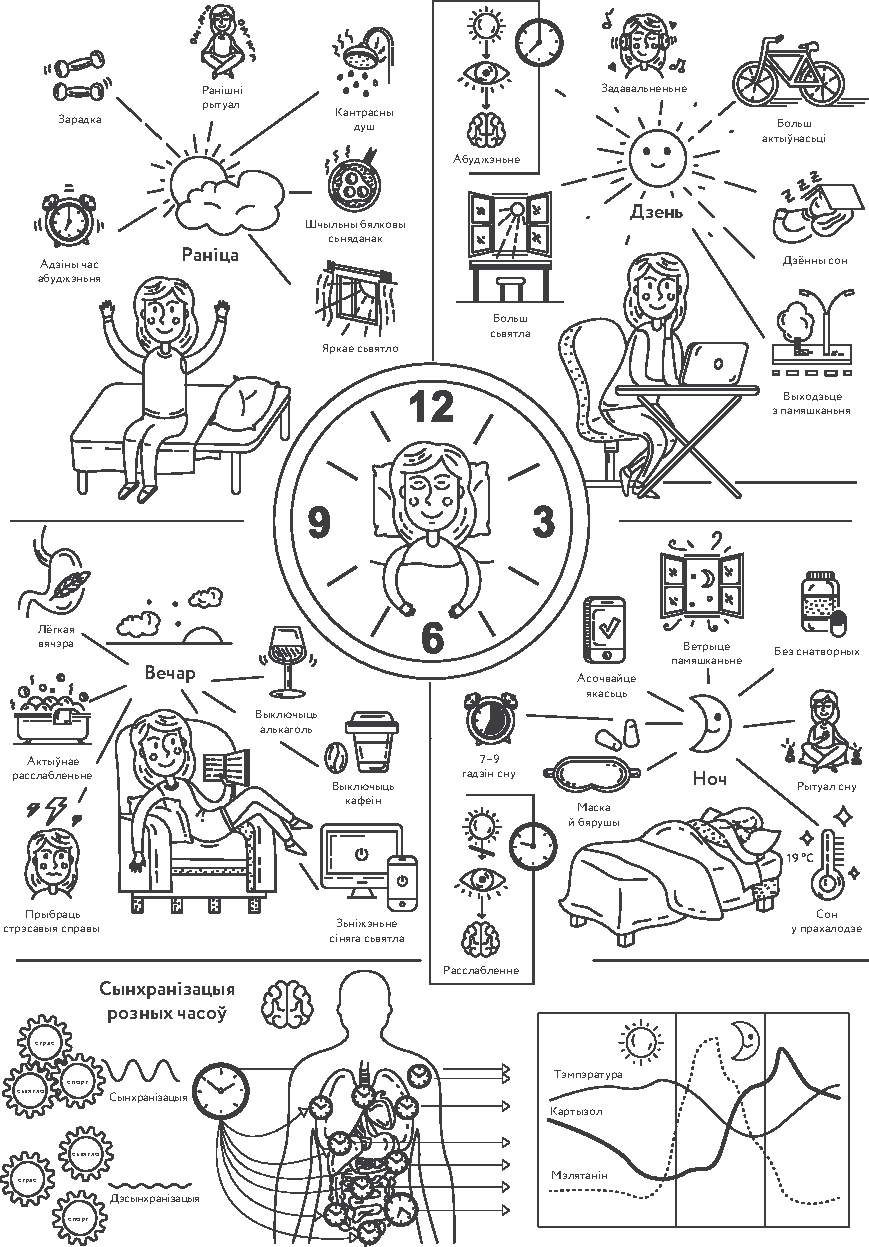
\includegraphics[width=\textwidth]{willpower/ch6/full.pdf}  
\end{figure}
